\documentclass[]{report}

\usepackage{graphicx}
\usepackage{float}
\usepackage{listings}
\usepackage{xcolor}

\definecolor{codegreen}{rgb}{0,0.6,0}
\definecolor{codegray}{rgb}{0.5,0.5,0.5}
\definecolor{codepurple}{rgb}{0.58,0,0.82}
\definecolor{backcolour}{rgb}{0.95,0.95,0.92}

\lstdefinestyle{mystyle}{
    backgroundcolor=\color{backcolour},   
    commentstyle=\color{codegreen},
    keywordstyle=\color{magenta},
    numberstyle=\tiny\color{codegray},
    stringstyle=\color{codepurple},
    basicstyle=\ttfamily\footnotesize,
    breakatwhitespace=false,         
    breaklines=true,                 
    captionpos=b,                    
    keepspaces=true,                 
    numbers=left,                    
    numbersep=5pt,                  
    showspaces=false,                
    showstringspaces=false,
    showtabs=false,                  
    tabsize=2
}

\lstset{style=mystyle}


\setcounter{secnumdepth}{1}
\setcounter{tocdepth}{1}

%opening
\title{Client-Side Many-Valued Context Scaling}
\author{Sebastian Benner}

\begin{document}

\maketitle

\tableofcontents

\chapter{Task}
Implementation of a client-side web-application to scale many-valued contexts in clojurescript using Reagent and Re-Frame. The CSS is done by using Bulma.

Up until now there was no easy to use interactive tool to scale many-valued contexts. These contexts are most commonly stored as comma-seperated values (.csv). In order to transform them into formal contexts and save them as such (.ctx) there are three scaling methods a tool must implement: nominal, ordinal and numeric scaling. All of them require completely different designs for the user interface in order to be intuitive. Additionally experienced users tend to skip most interfaces and might want to work directly with the data, the tool should provide such an option.

\section{Timetable}
There are several major steps to be taken in order to complete such a task:
\begin{enumerate}
	\item A basic skeleton which reads in .csv files, scales them all in the most basic way and exports the resulting context as file. (2-3 weeks)
	\item Implement functions for all types (nominal, ordinal and numeric) of scaling. (1-2 weeks)
	\item Build an interface for the user to manipulate the scaling for each attribute with some helpful statistics. (3-4 weeks)
	\item Export a config-file which can later be imported to quickly change the method of scaling. (1 week)
	\item Implement algorithms to suggest more optimal scaling and minimize user input. (1-2 weeks)
	\item Give more detailed statistics and graphs for each attribute. (optional)
\end{enumerate}
Overall time for implementation: 8-12 weeks. The remaining weeks are to be used for the written part and presentation.


\chapter{Mock-Up}
What follows is a basic collection of all screens created during the design process. As such they may be subject to change later one but all of them serve as basic guideline for the features each screen must include. They are ordered in the same way a user would experience them: First the data is uploaded in section 1, afterwards all attributed to be scaled are selected. The third and fourth panel then are used to scaled and export the final context respectively.

\section{Import-Panel}
\begin{figure}[H]
	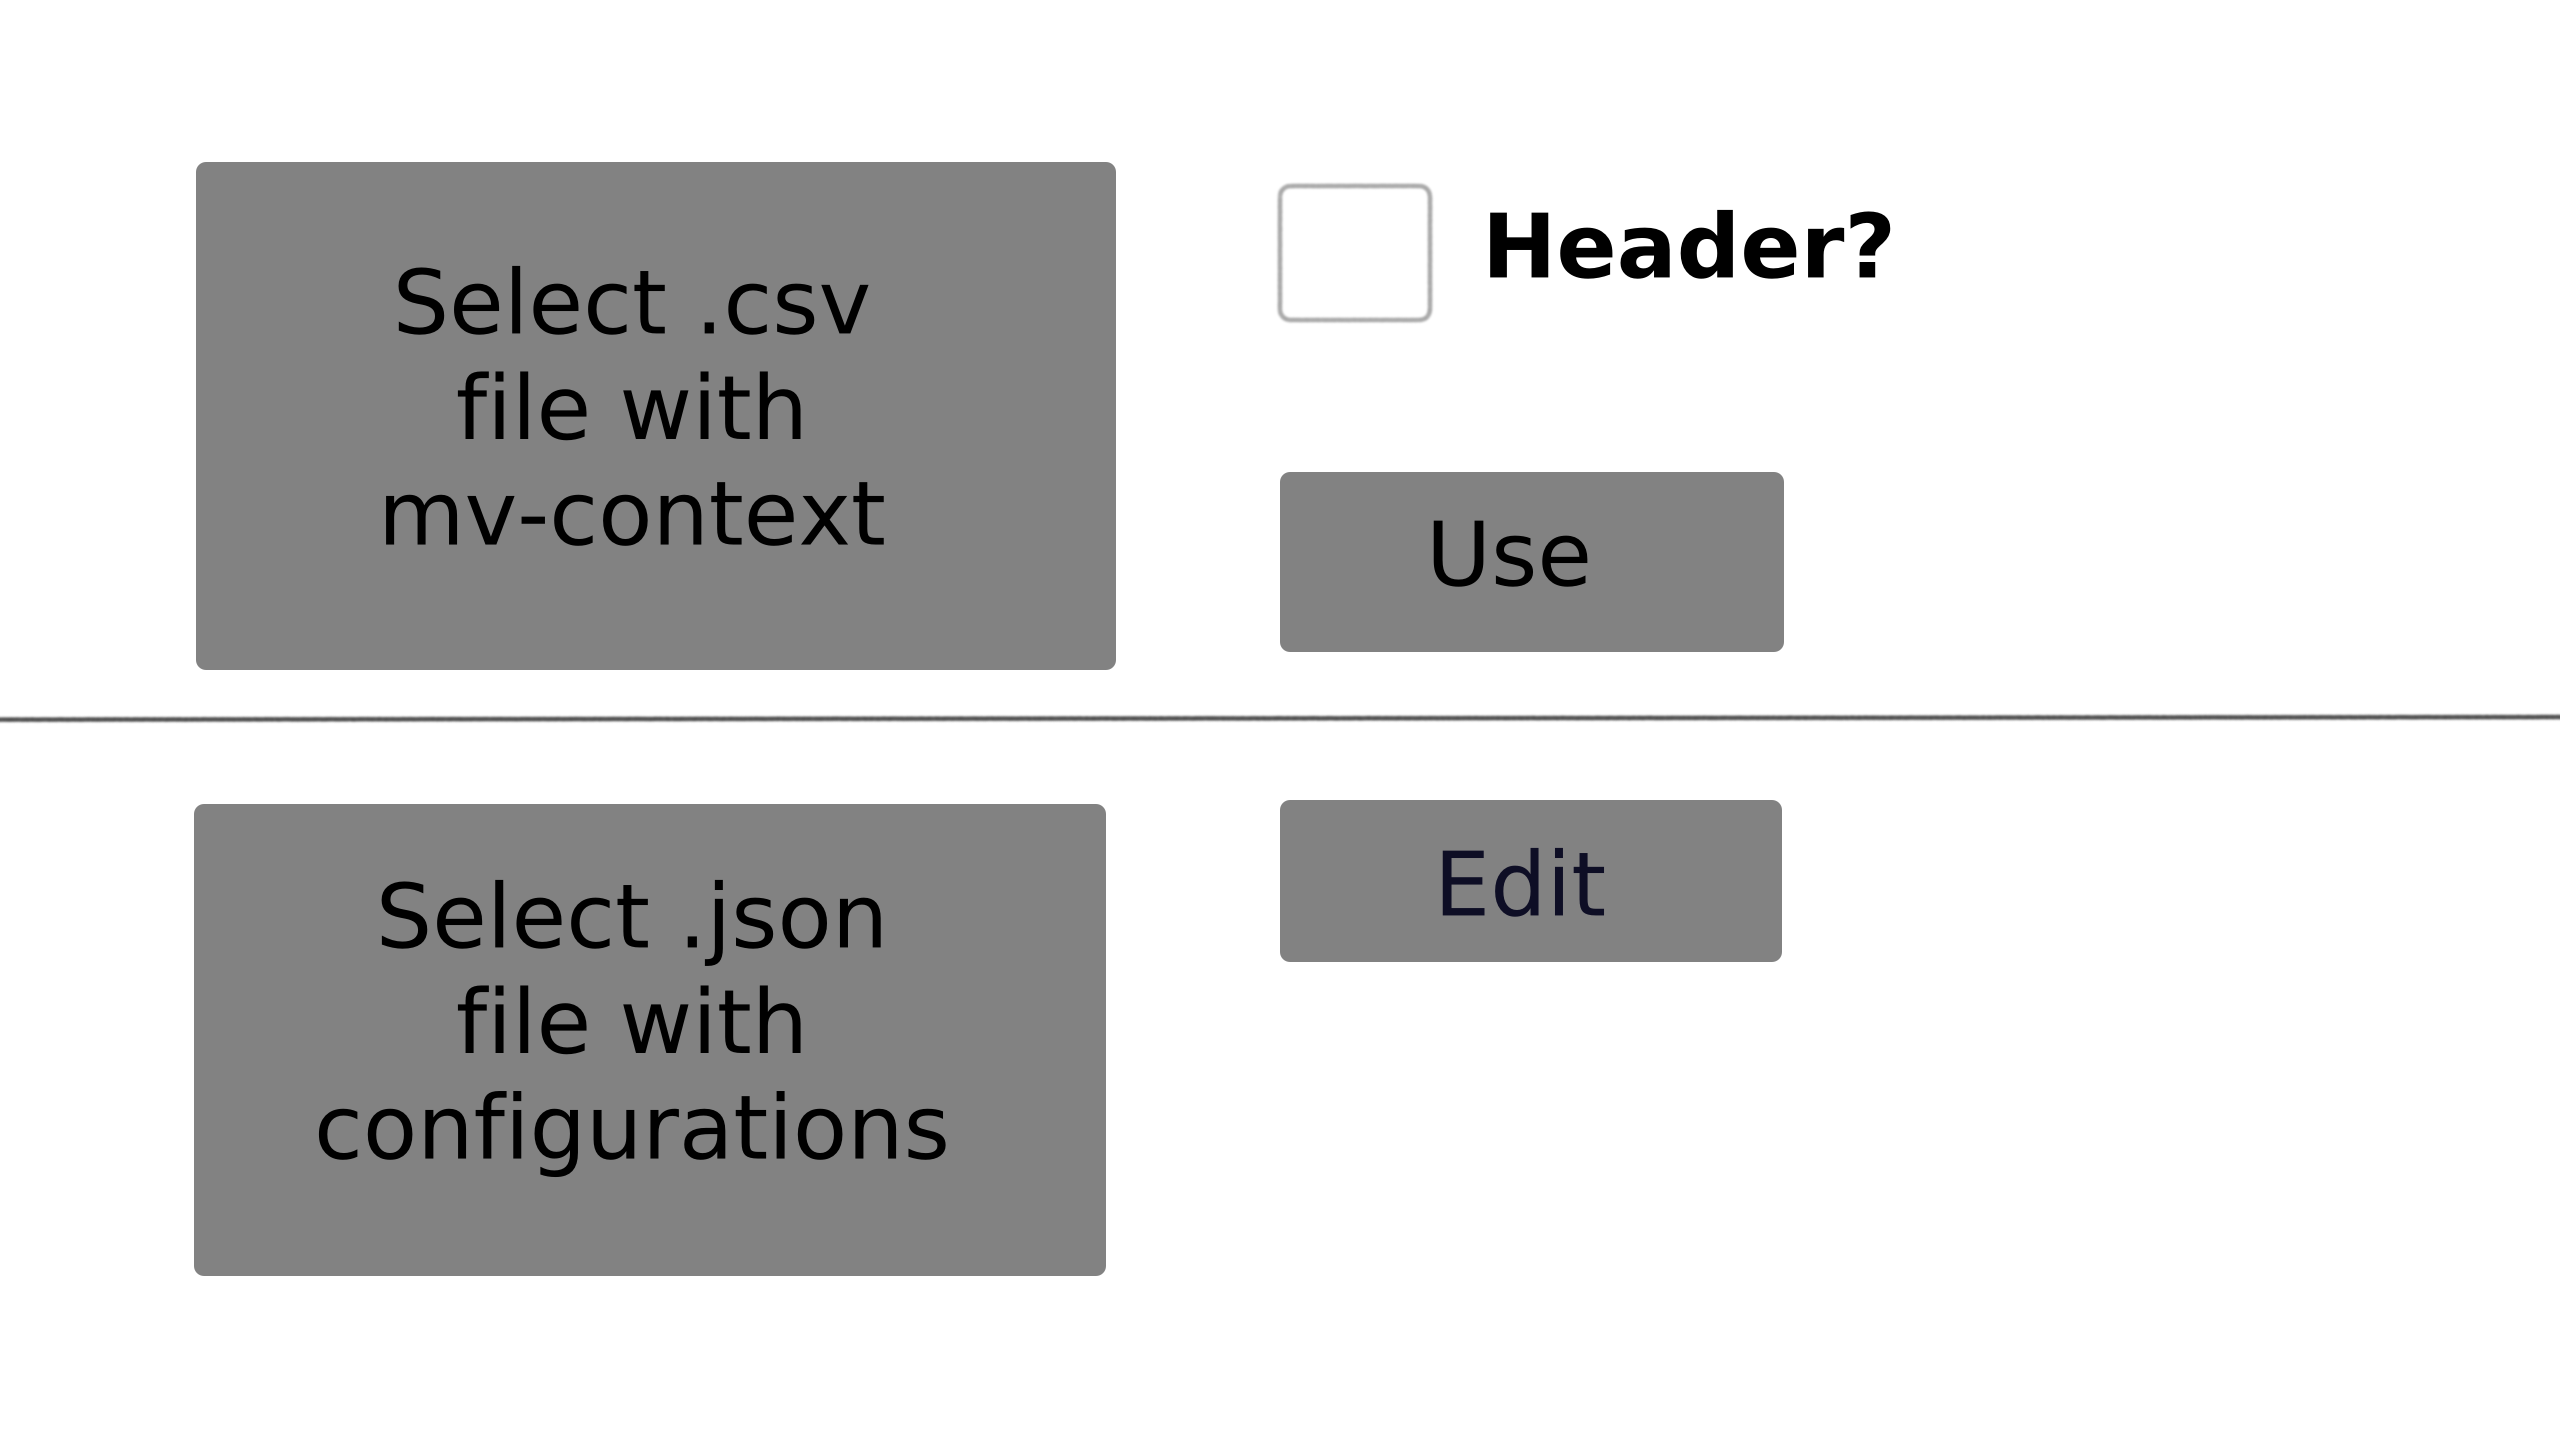
\includegraphics[width=\linewidth]{mock_up/panel-1.png}
	\caption{The panel to select files (both versions)}
	\label{fig:p1}
\end{figure}

\subsection{Features}
\begin{itemize}
	\item Select any local .csv file with a mv-context
	\item Checkbox to mark existence of a header line
	\item Different input box to instead reuse a .json file with an old configuration
	\item Button to second panel
\end{itemize}

\newpage
\section{Selection-Panel}
\begin{figure}[H]
	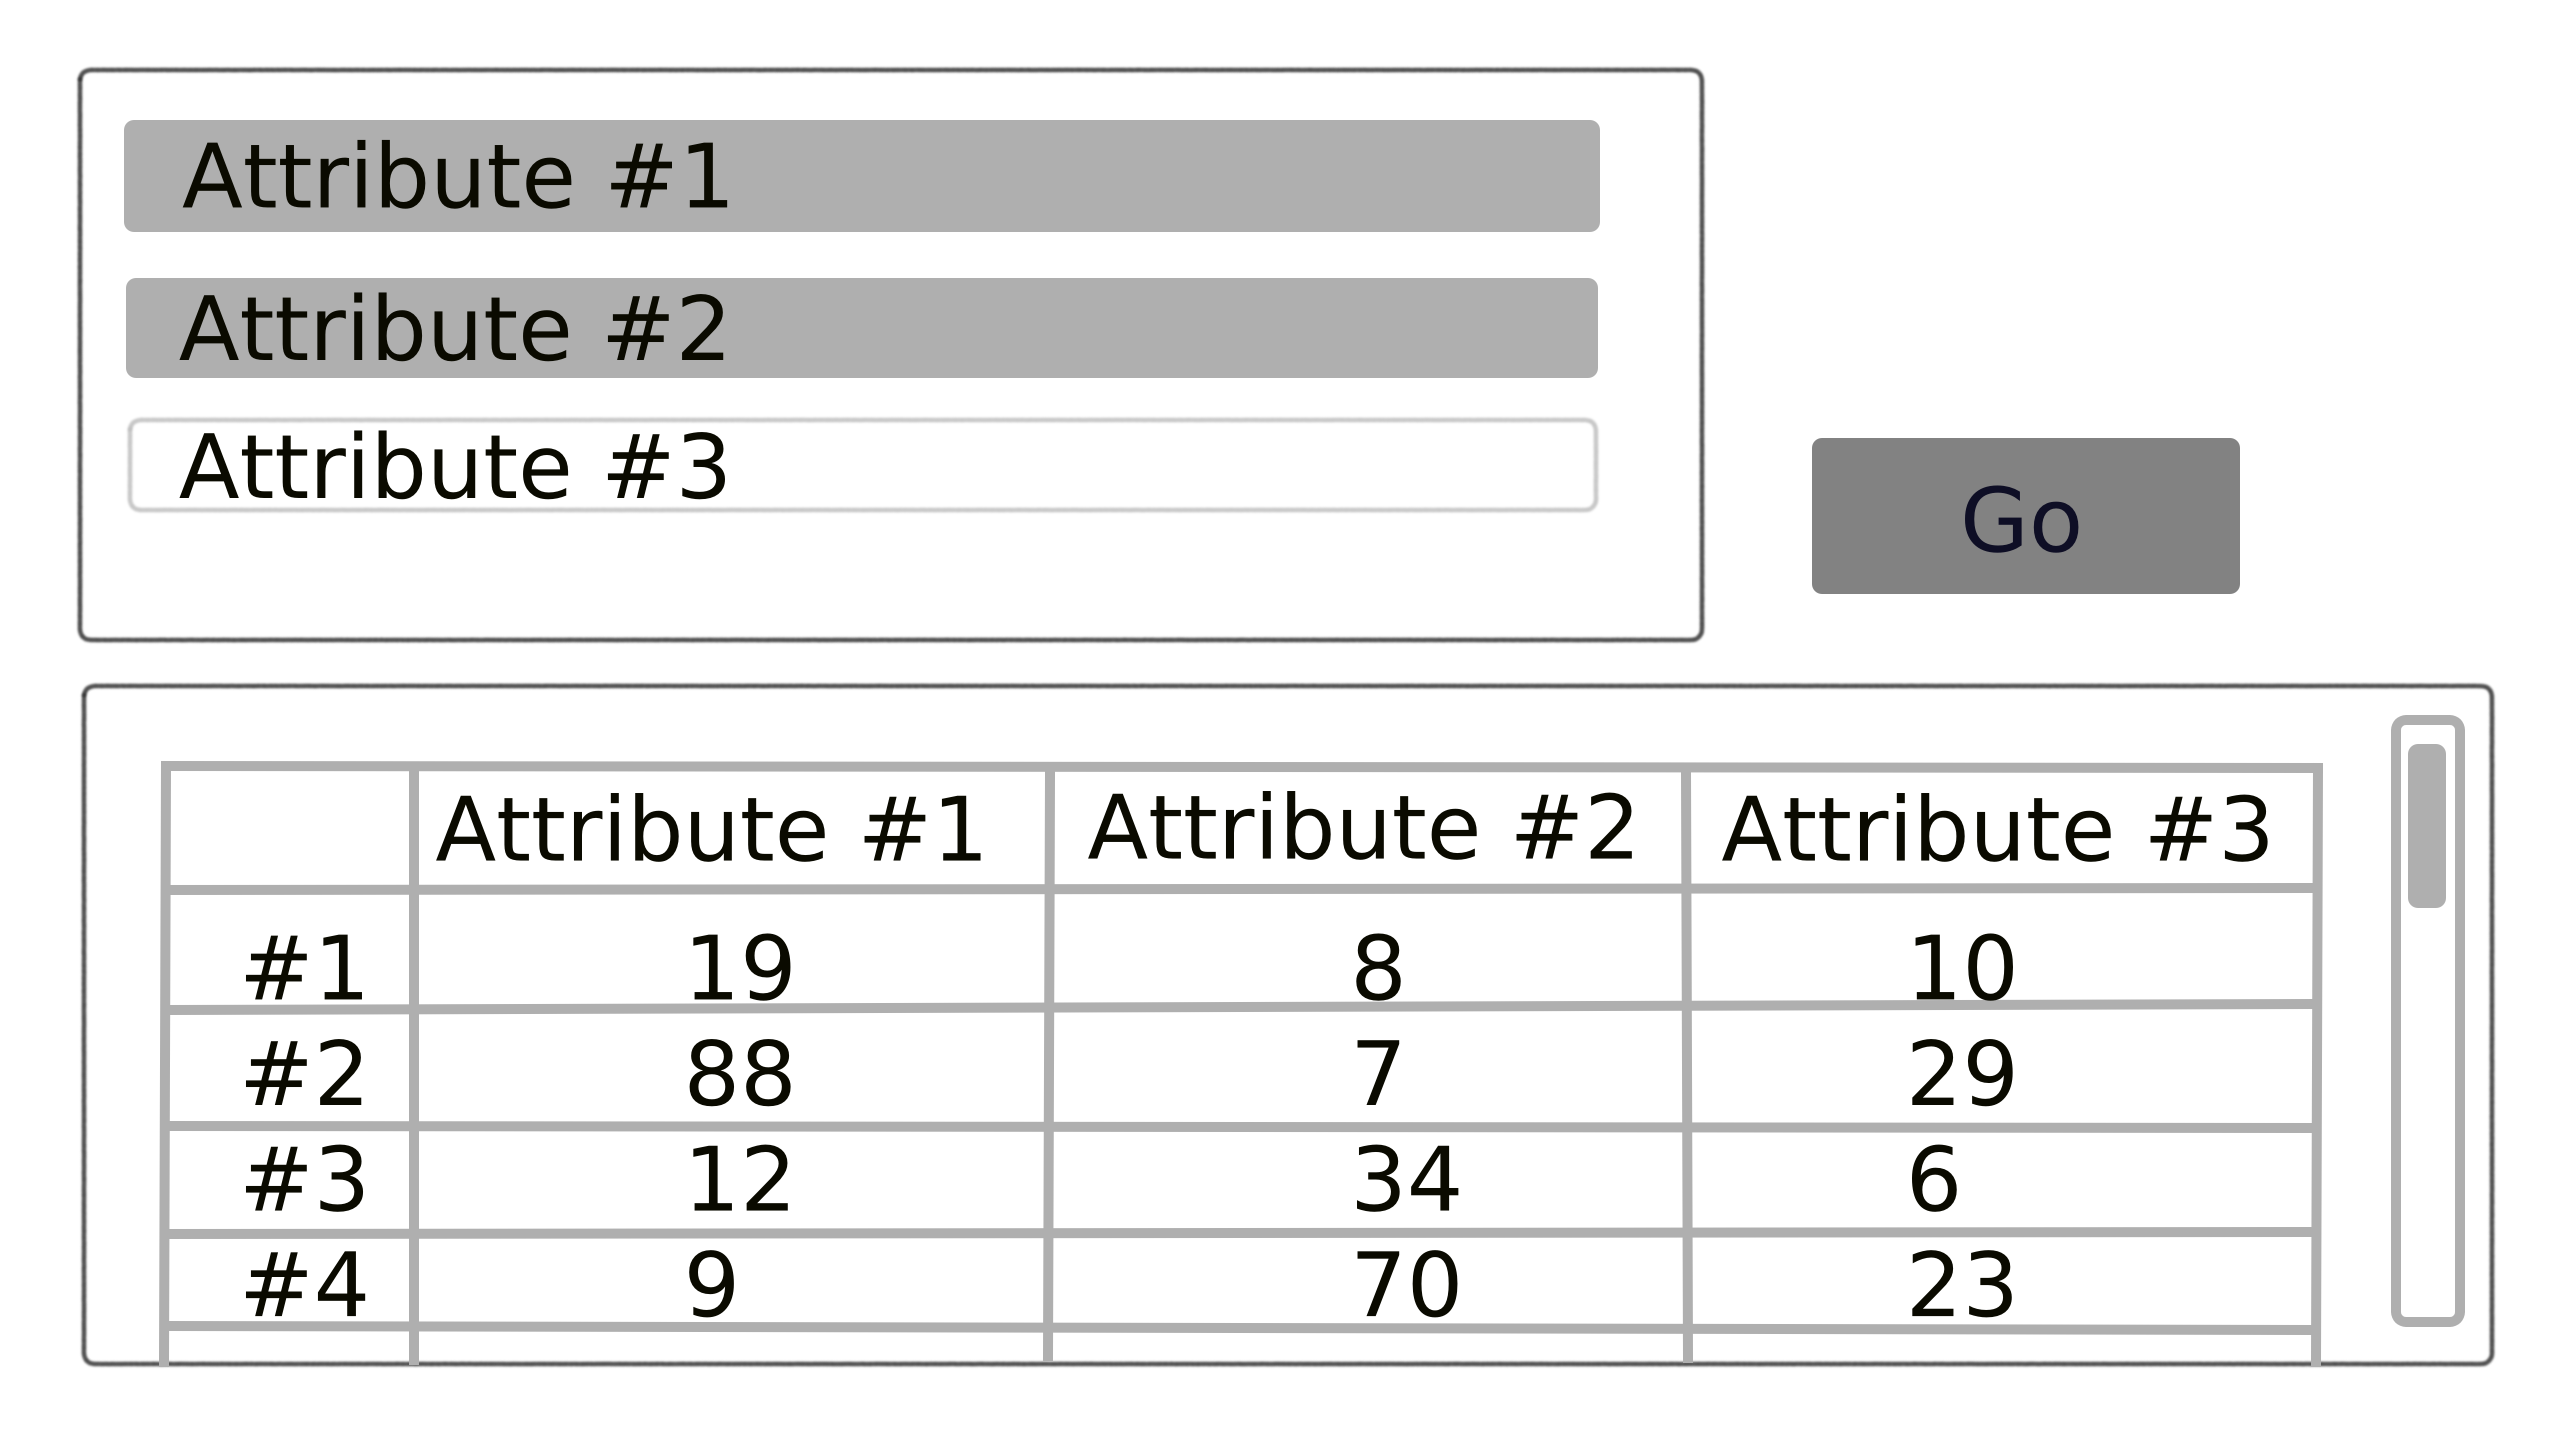
\includegraphics[width=\linewidth]{mock_up/panel-2.png}
	\caption{Preselection panel}
	\label{fig:p2}
\end{figure}

\subsection{Features}
\begin{itemize}
	\item Select all Attributes (multi-select input) to scale (gray) and to exclude (white)
	\item Preview of the context in scroll-able box (x and y axis)
	\item Button to third panel
\end{itemize}

\newpage
\section{Scaling-Panel}
\begin{figure}[H]
	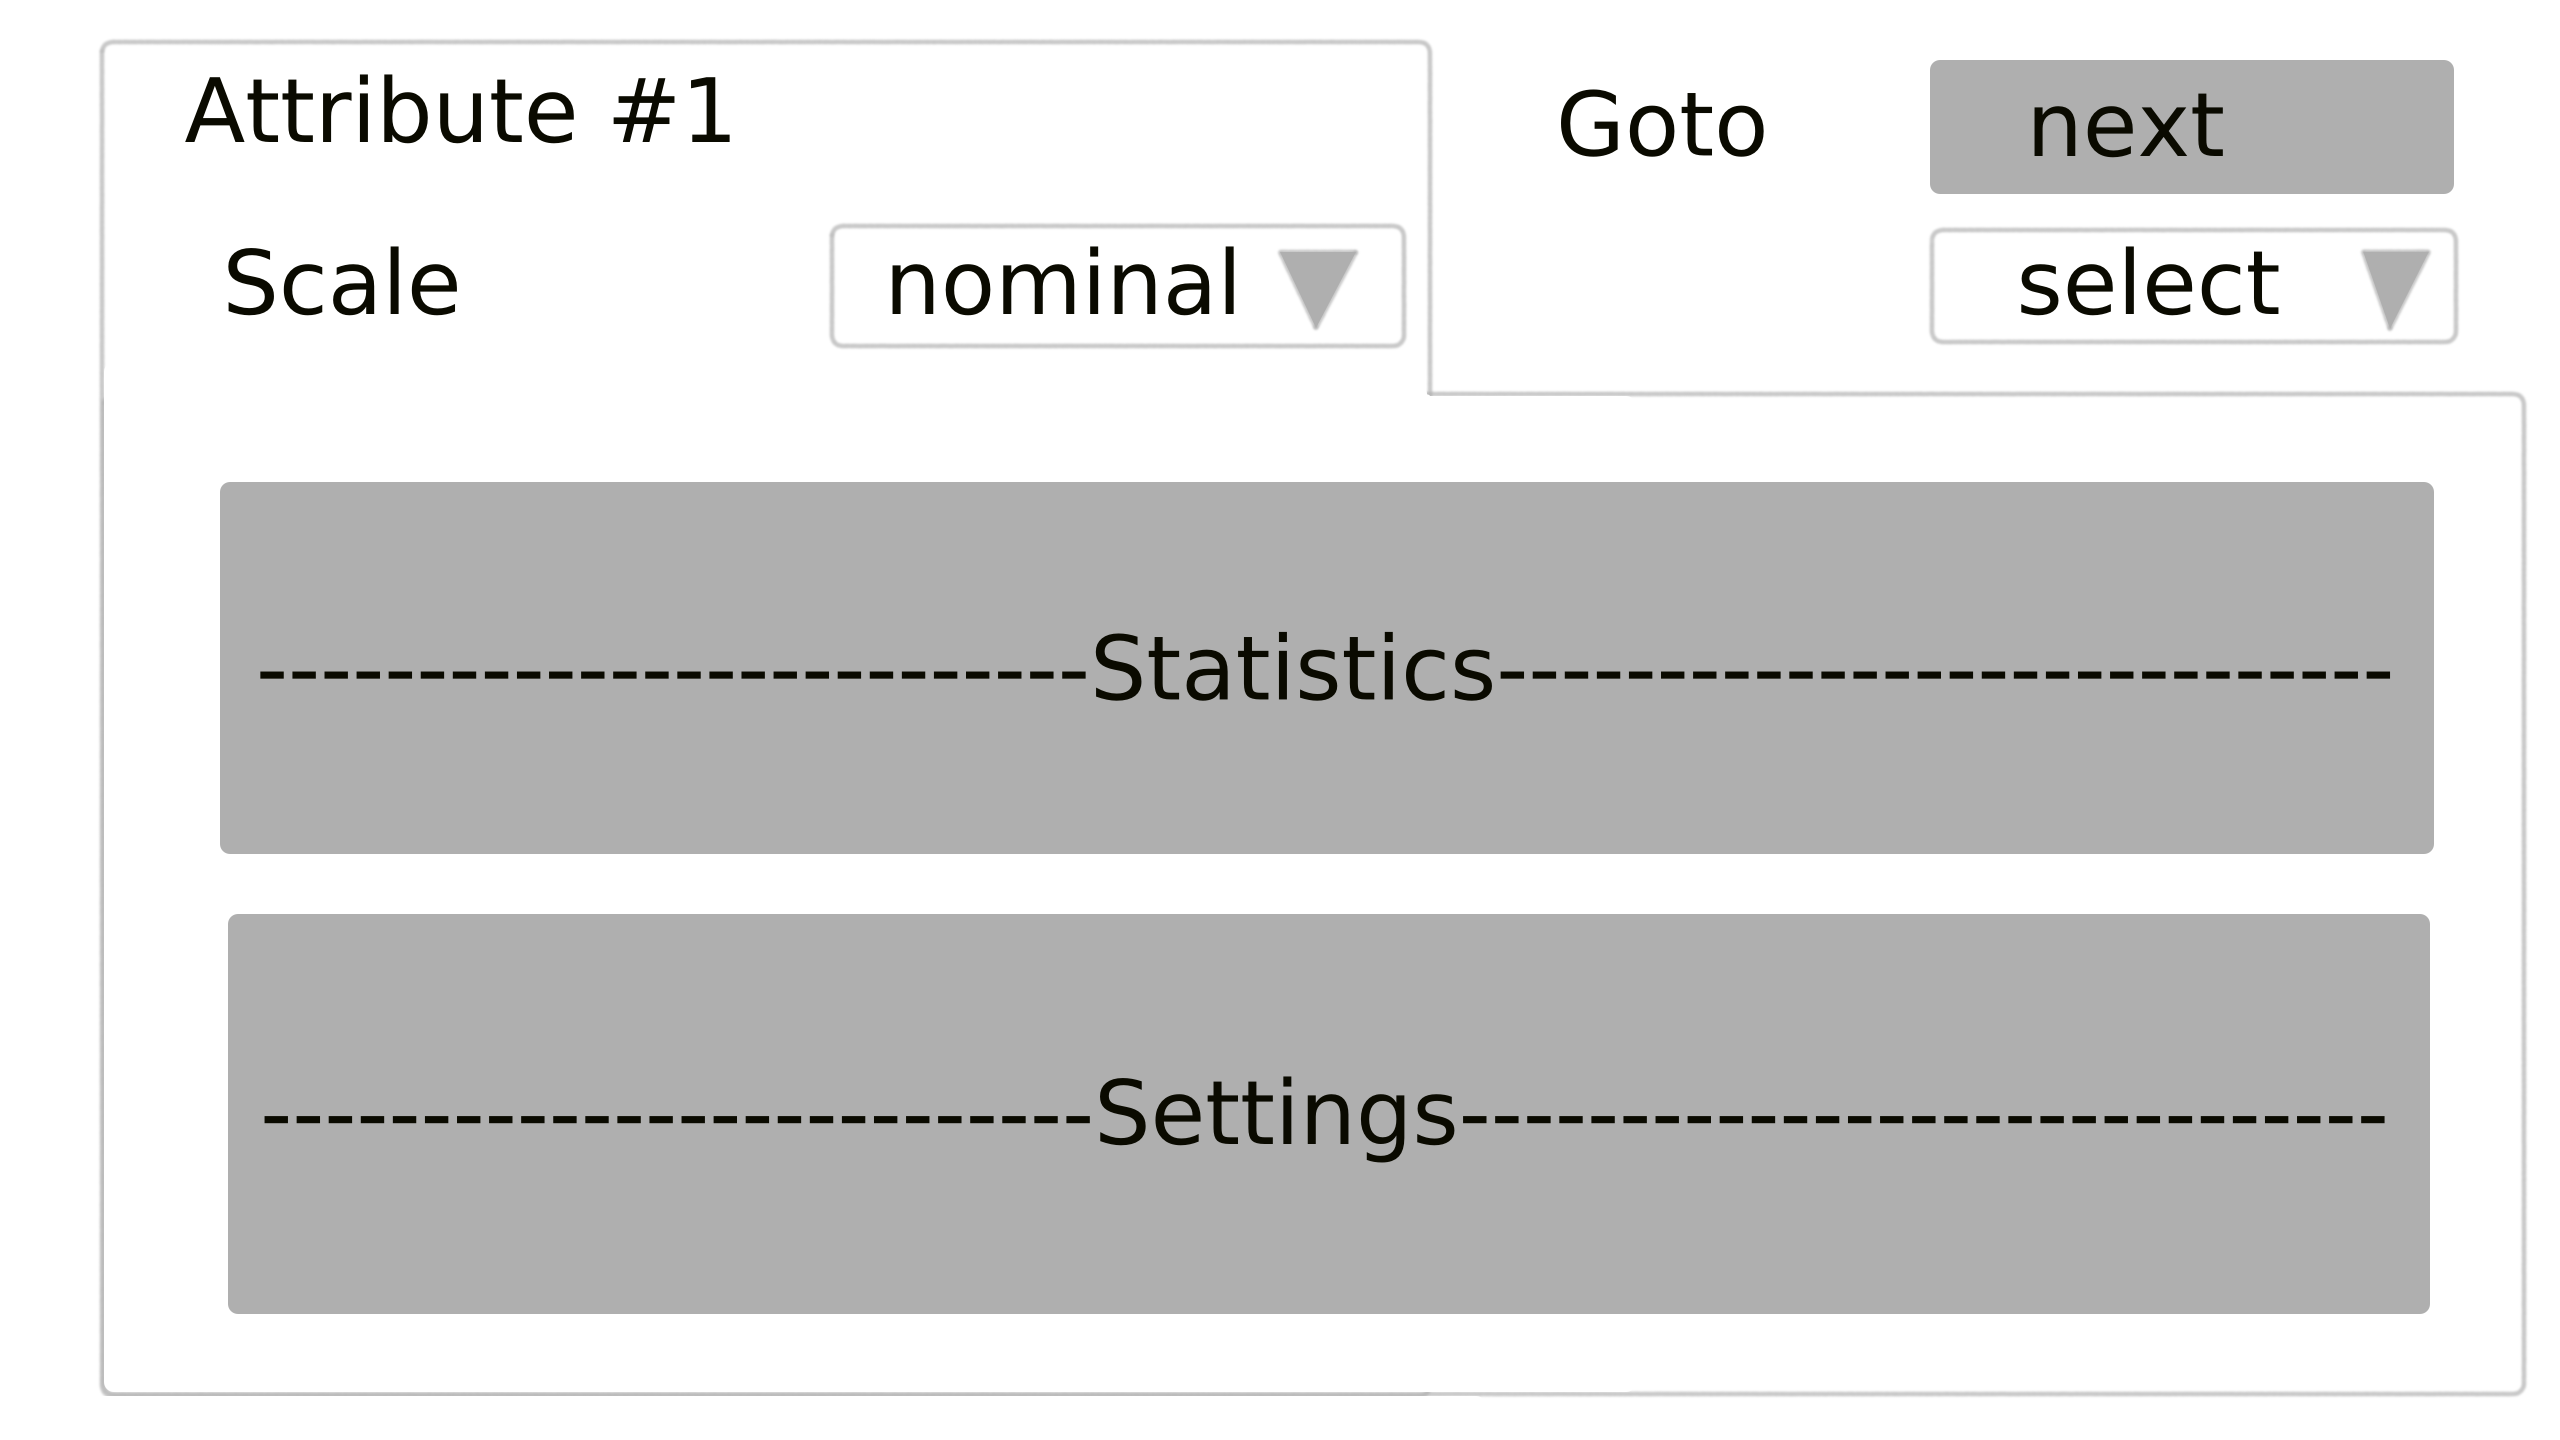
\includegraphics[width=\linewidth]{mock_up/panel-3.png}
	\caption{Scaling panel}
	\label{fig:p2}
\end{figure}
\begin{itemize}
	\item Preselected scaling option for each attribute
	\item Option to choose different measurement levels (ordinal and numeric)
	\item Descriptive statistics for values of each attribute
	\item Settings to change scaling
	\item Button to iterate attributes
	\item Selection to jump between attributes
\end{itemize}

\subsection{Statistics}
\begin{figure}[H]
	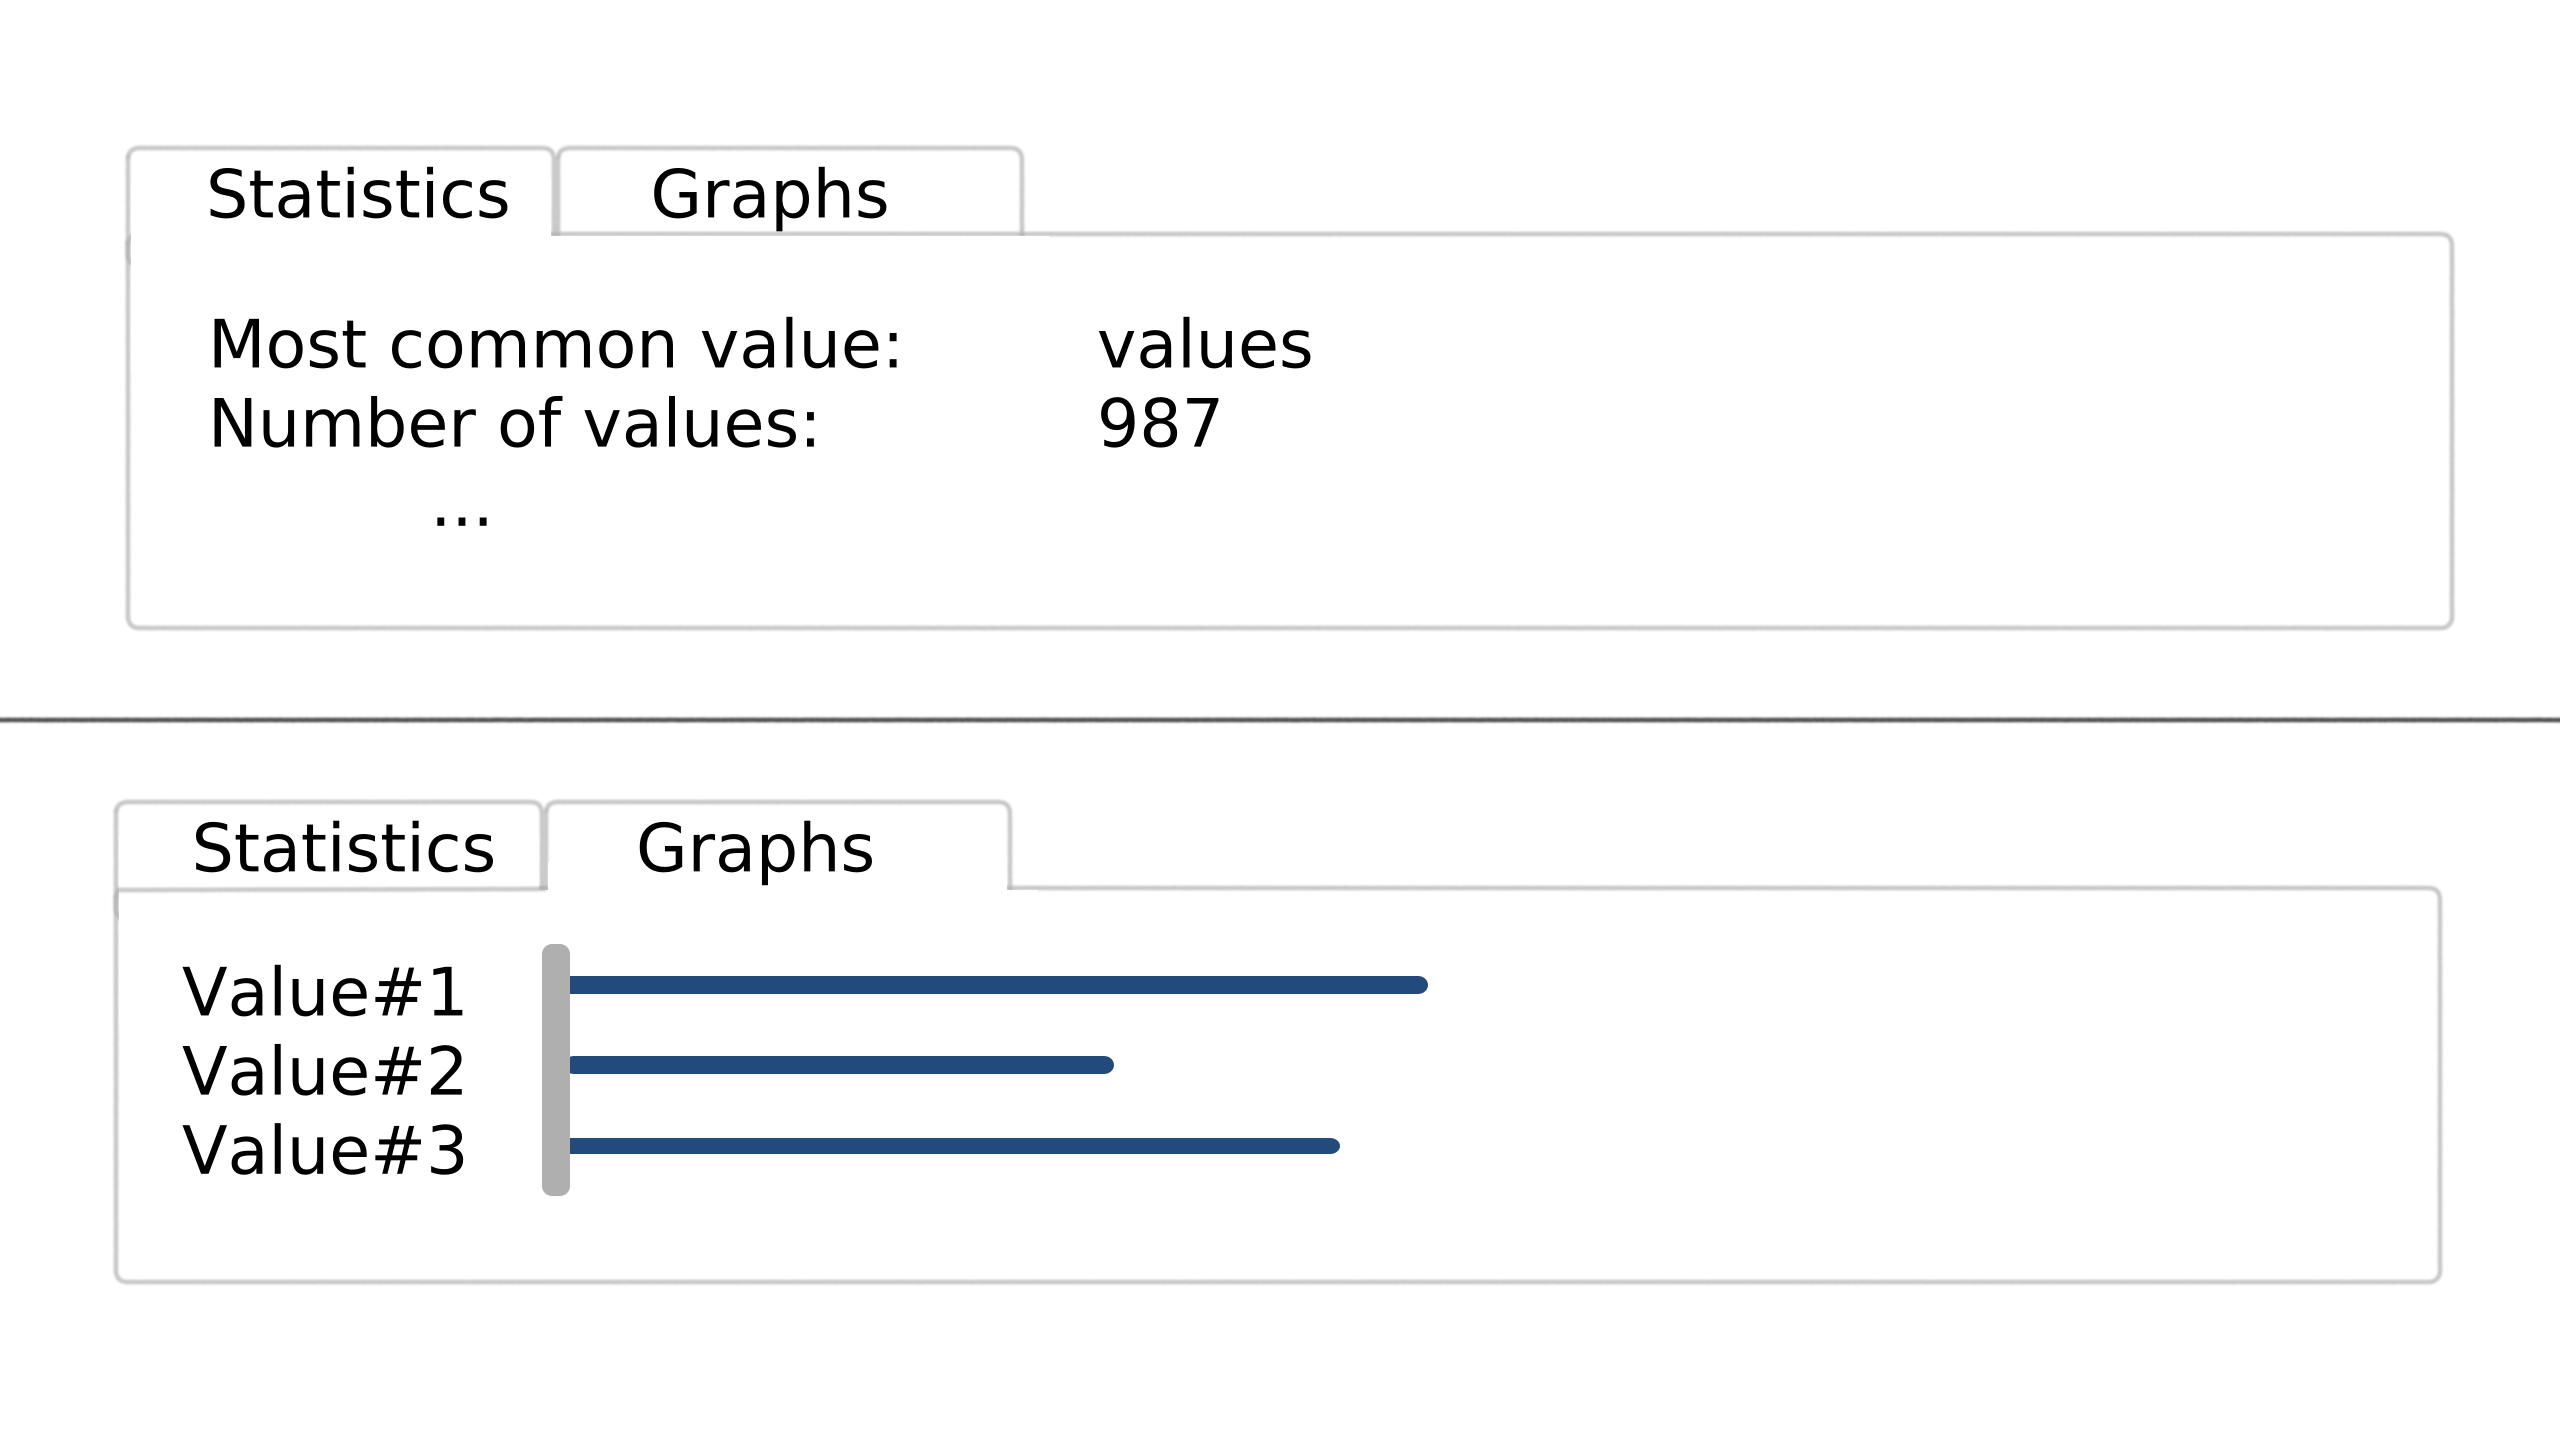
\includegraphics[width=\linewidth]{mock_up/stat.png}
	\caption{Statistics panel}
	\label{fig:s1}
\end{figure}
\begin{itemize}
	\item Based on data type and measure: mean, median, list of all values , most common element etc.
	\item Distribution graphs
\end{itemize}

\newpage
\subsection{Settings}
\begin{itemize}
	\item Nominal
		\begin{itemize}
		\item Entirely automatic
		\end{itemize}	    
	\item Ordinal
		\begin{figure}[H]
			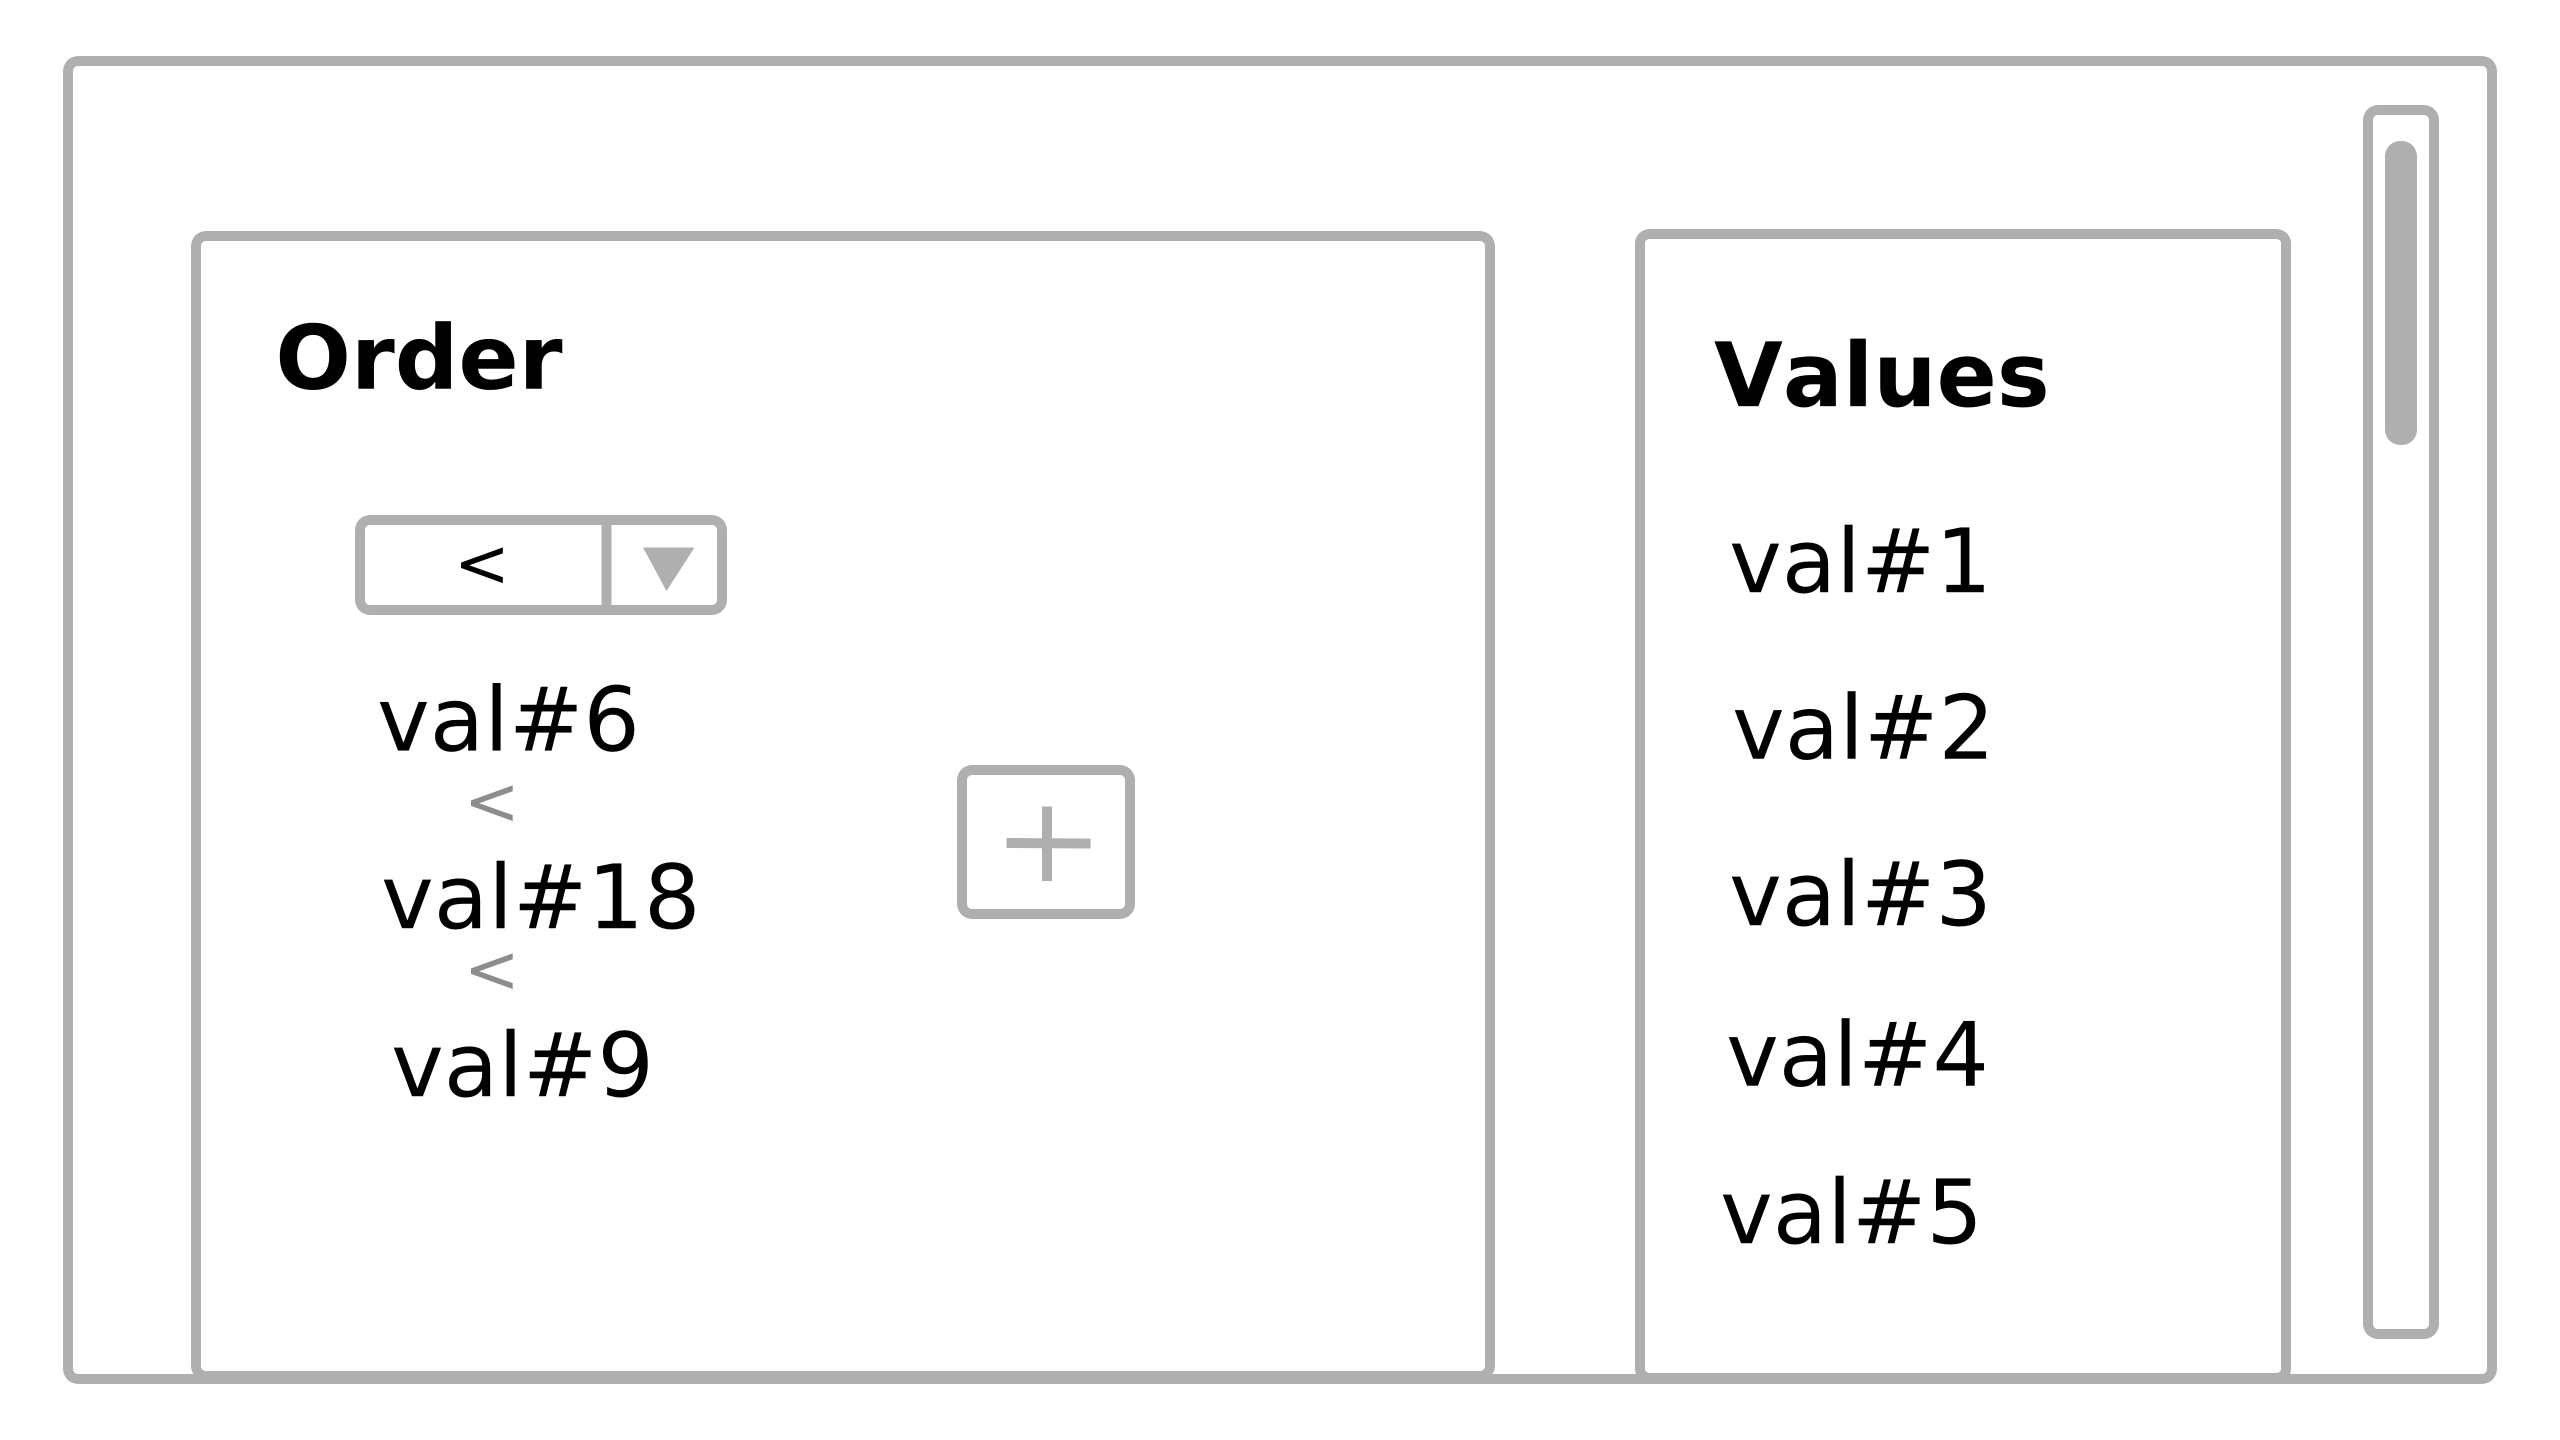
\includegraphics[width=\linewidth]{mock_up/ord-2.png}
			\caption{Drag and Drop Version}
			\label{fig:o1}
		\end{figure}
		\begin{itemize}
			\item Sort values with drag and drop
			\item Different incomparable groups
			\item Different types of order
			\item All unused values are scaled nominally 
		\end{itemize}
		\begin{figure}[H]
			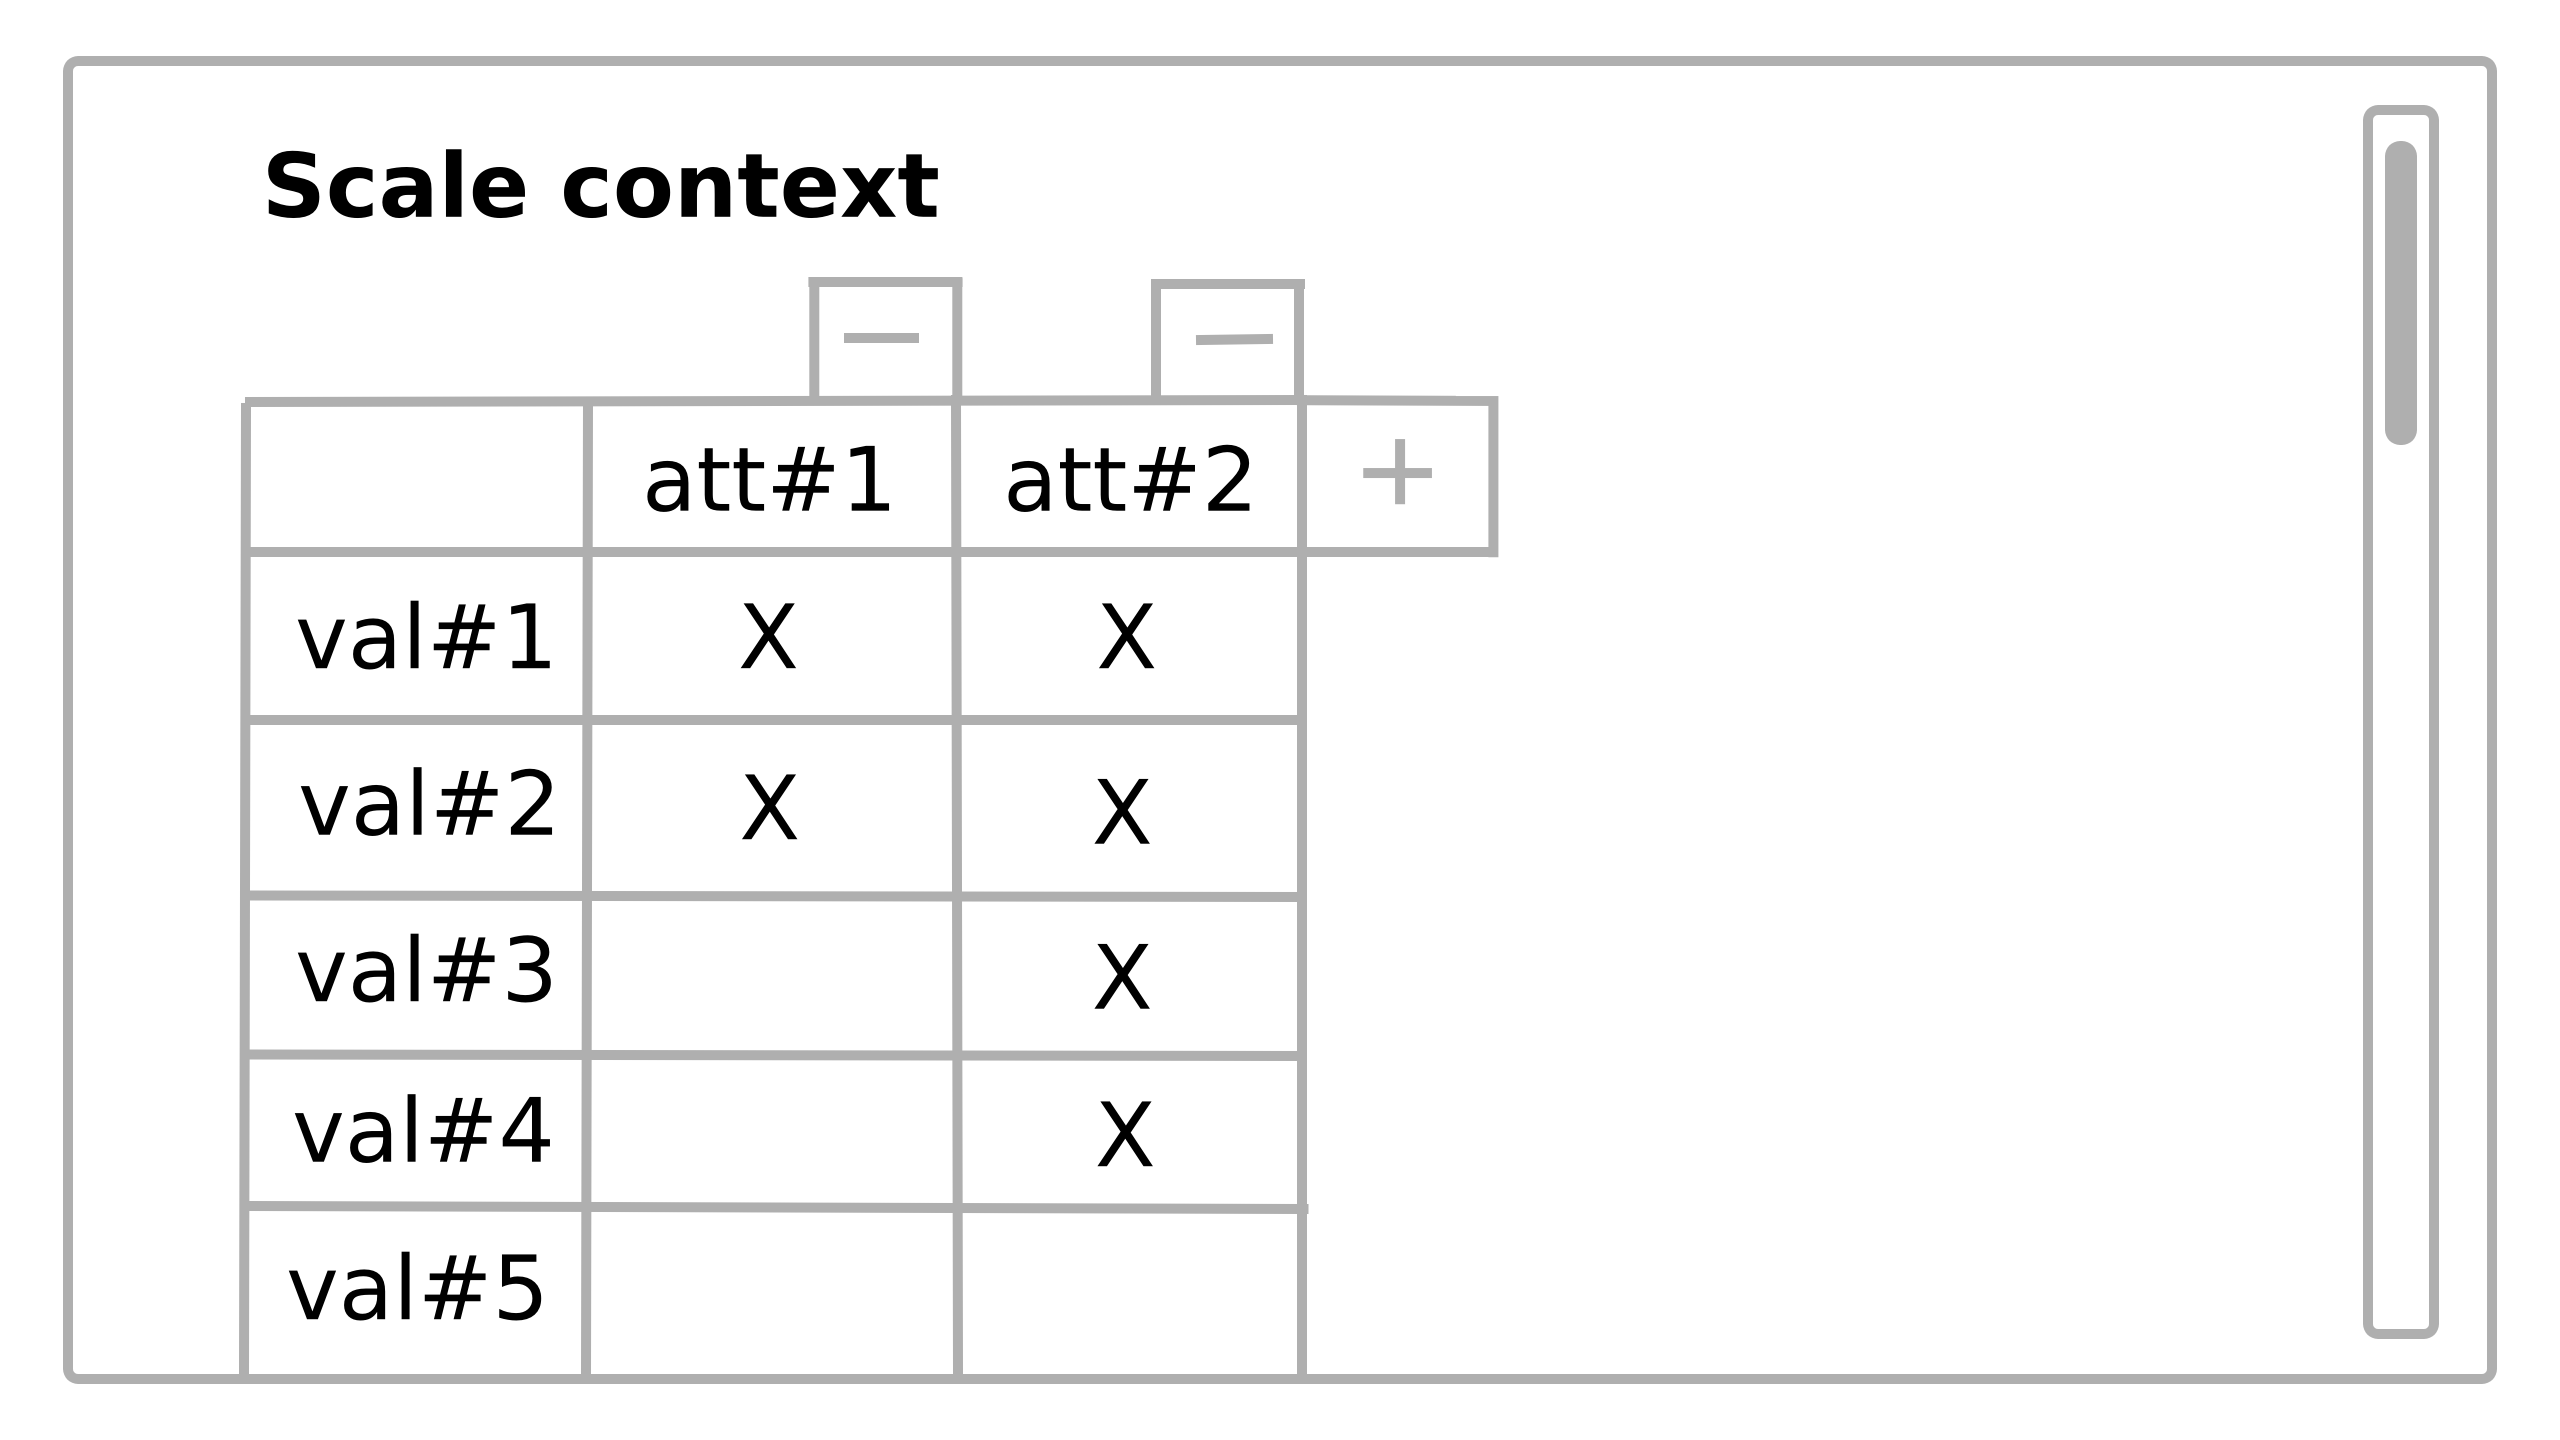
\includegraphics[width=\linewidth]{mock_up/ord-1.png}
			\caption{Custom context}
			\label{fig:o2}
		\end{figure}
		\begin{itemize}
			\item Option to edit scale context directly
			\item Add and remove rows
		\end{itemize}
	\item Numeric
		\begin{figure}[H]
			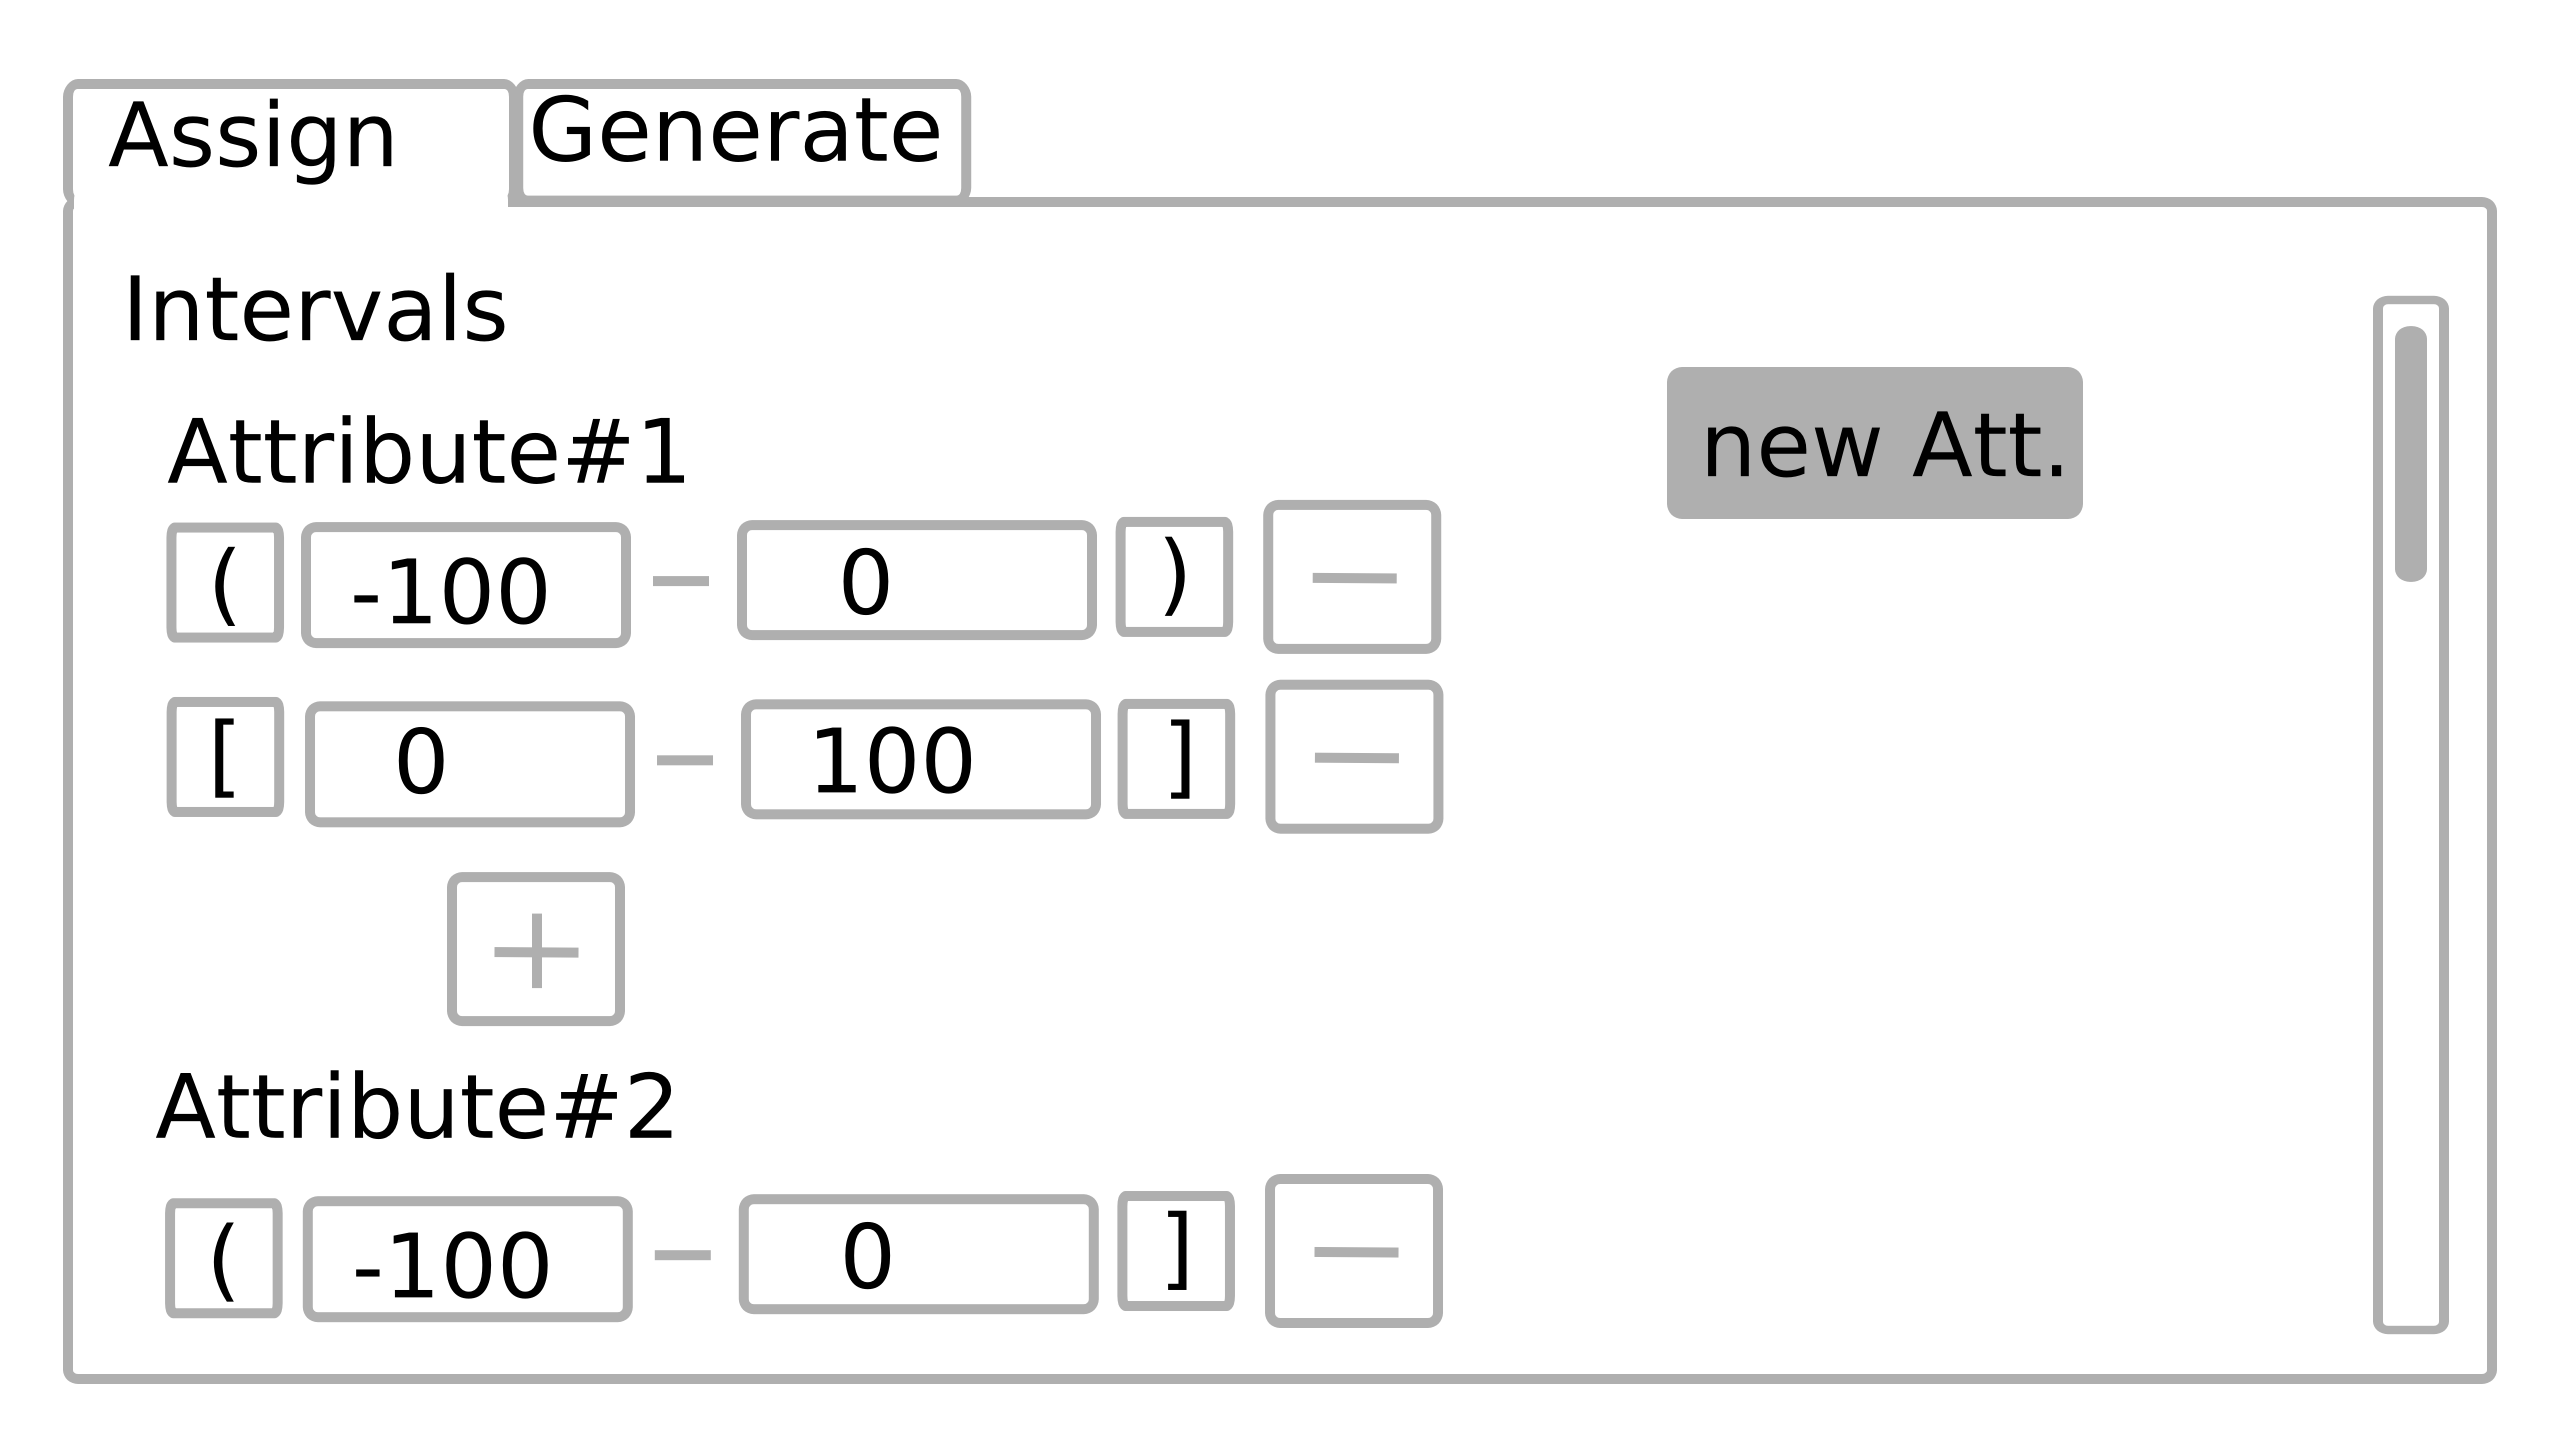
\includegraphics[width=\linewidth]{mock_up/num.png}
			\caption{Custom intervals}
			\label{fig:n1}
		\end{figure}
	    \begin{itemize}
	    	\item Use predefined intervals with custom amount
	    	\begin{figure}[H]
	    		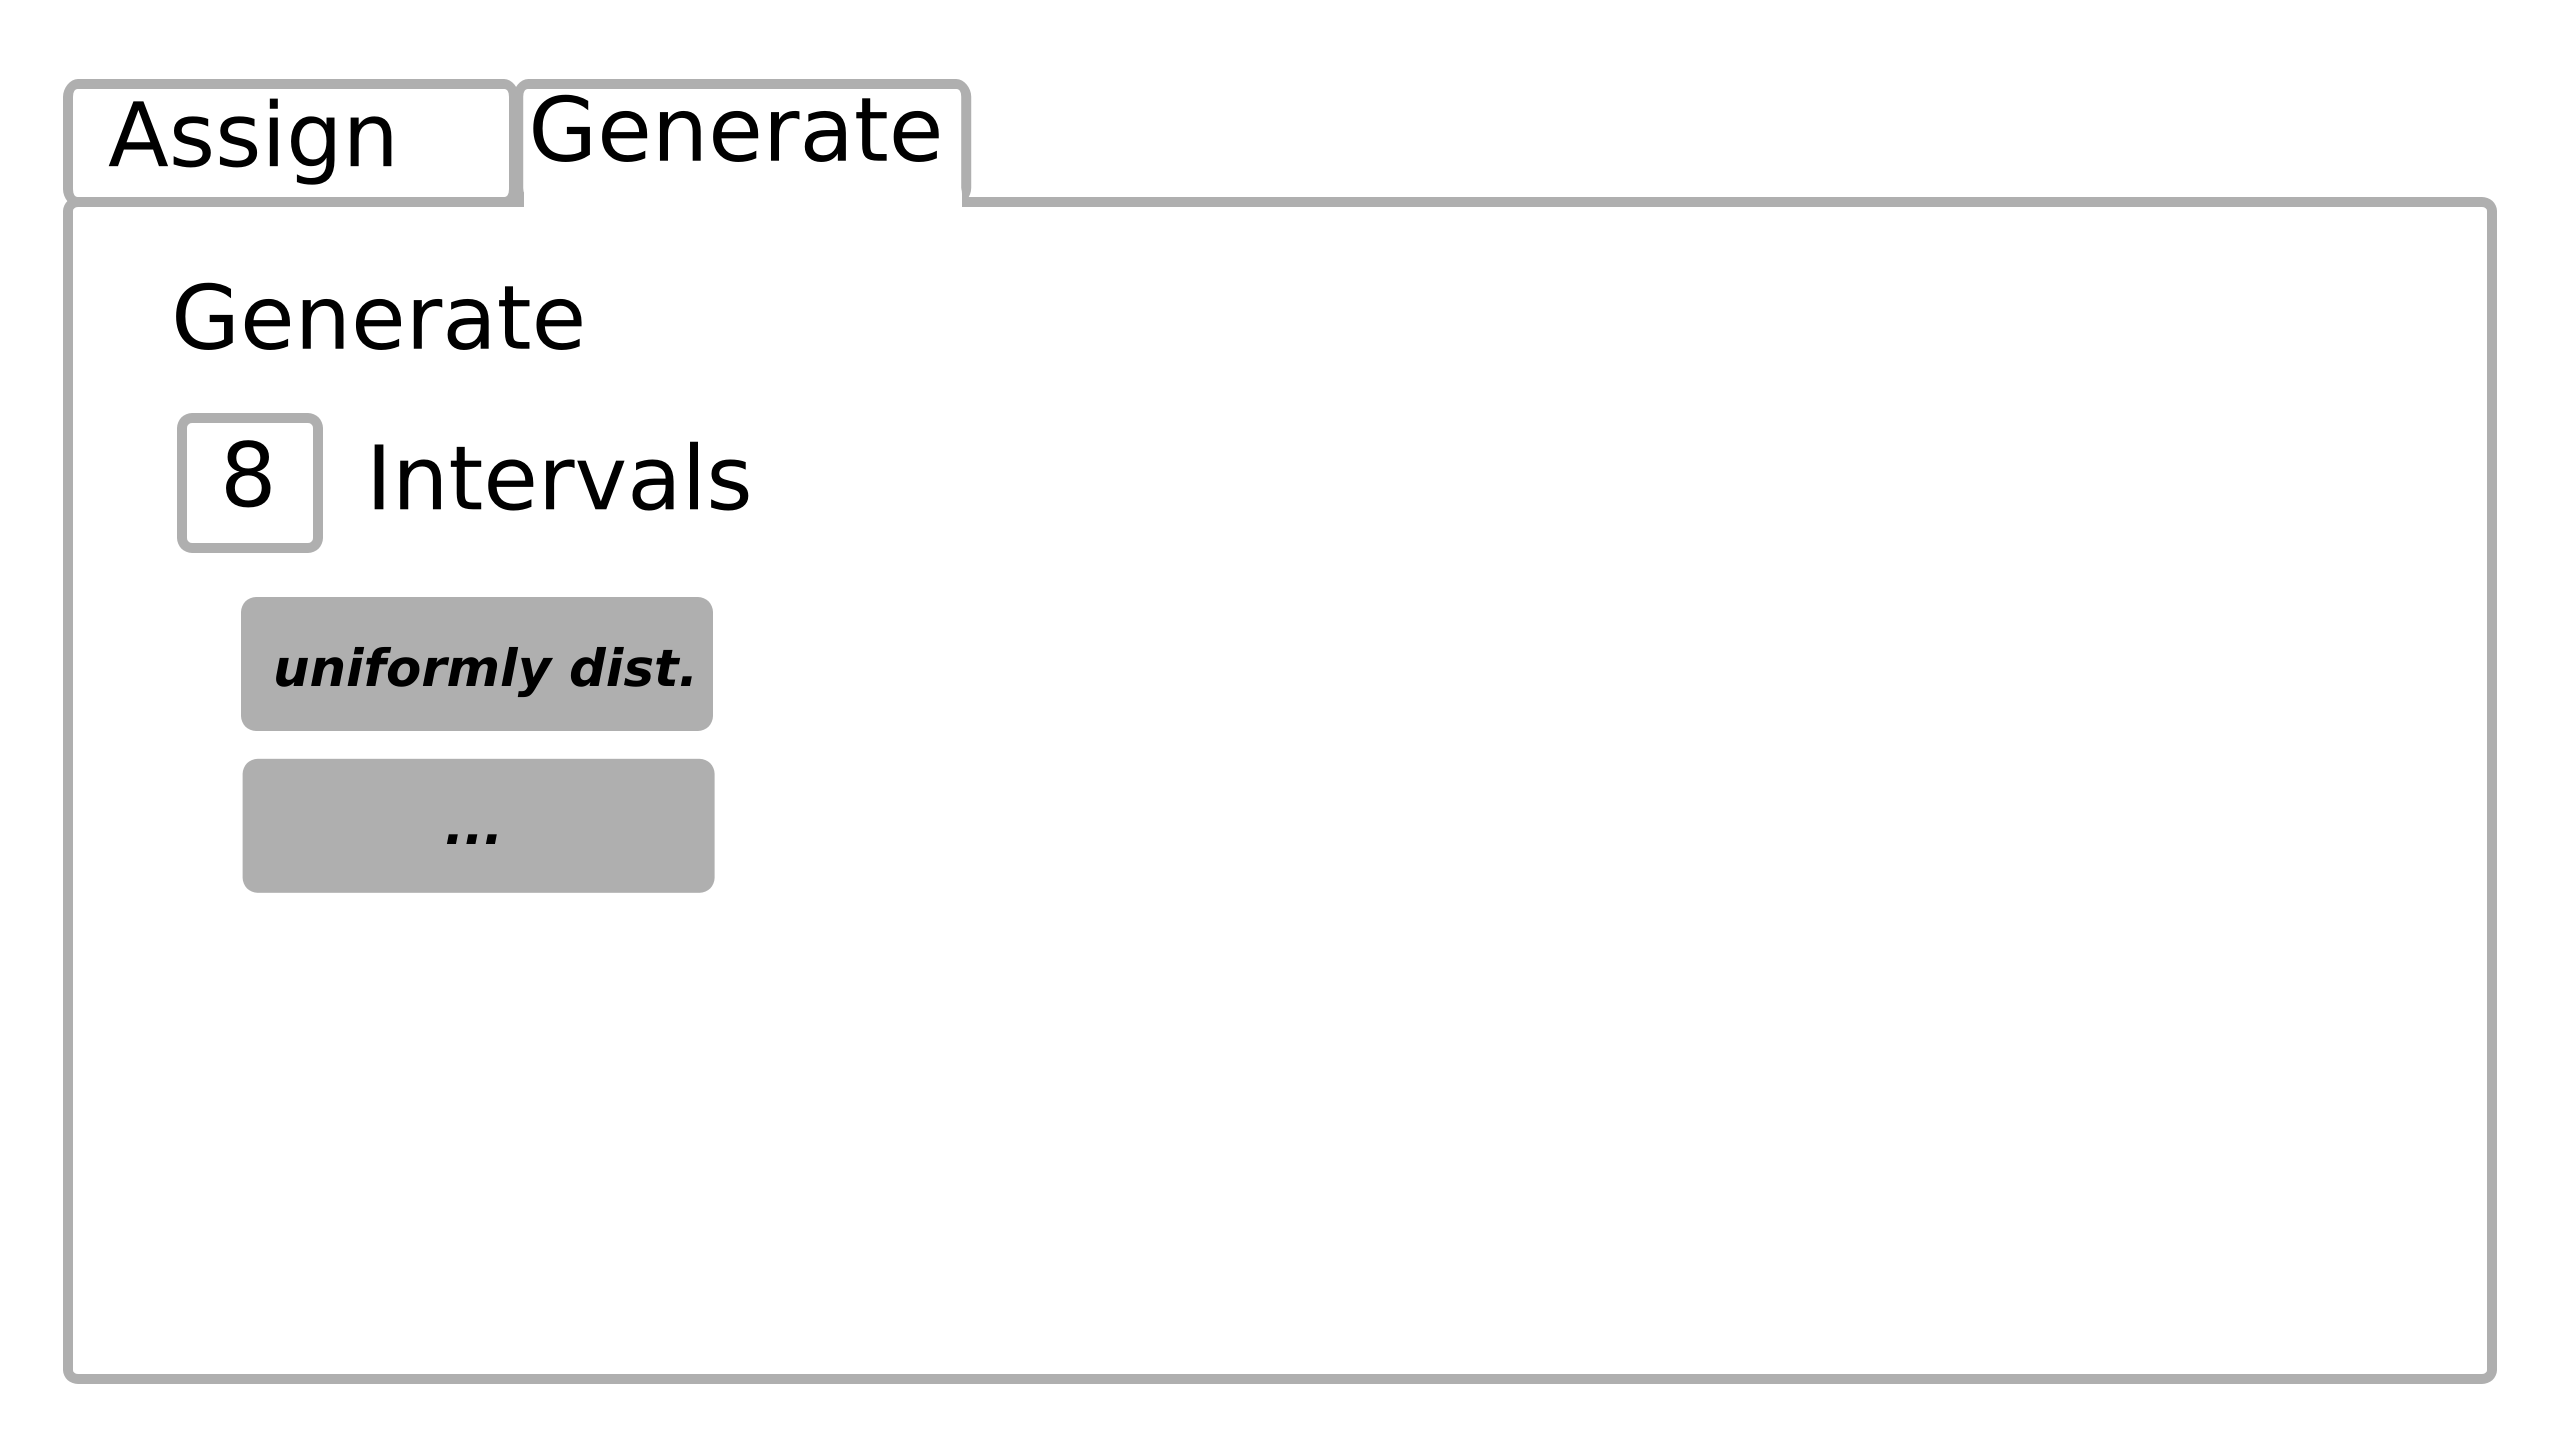
\includegraphics[width=\linewidth]{mock_up/num_gen.png}
	    		\caption{Generate predefined intervals}
	    		\label{fig:n1}
	    	\end{figure}
	    	\item Generate custom intervals
	    \end{itemize}
\end{itemize}

\newpage
\section{Export-Panel}
	\begin{itemize}
		\begin{figure}[H]
			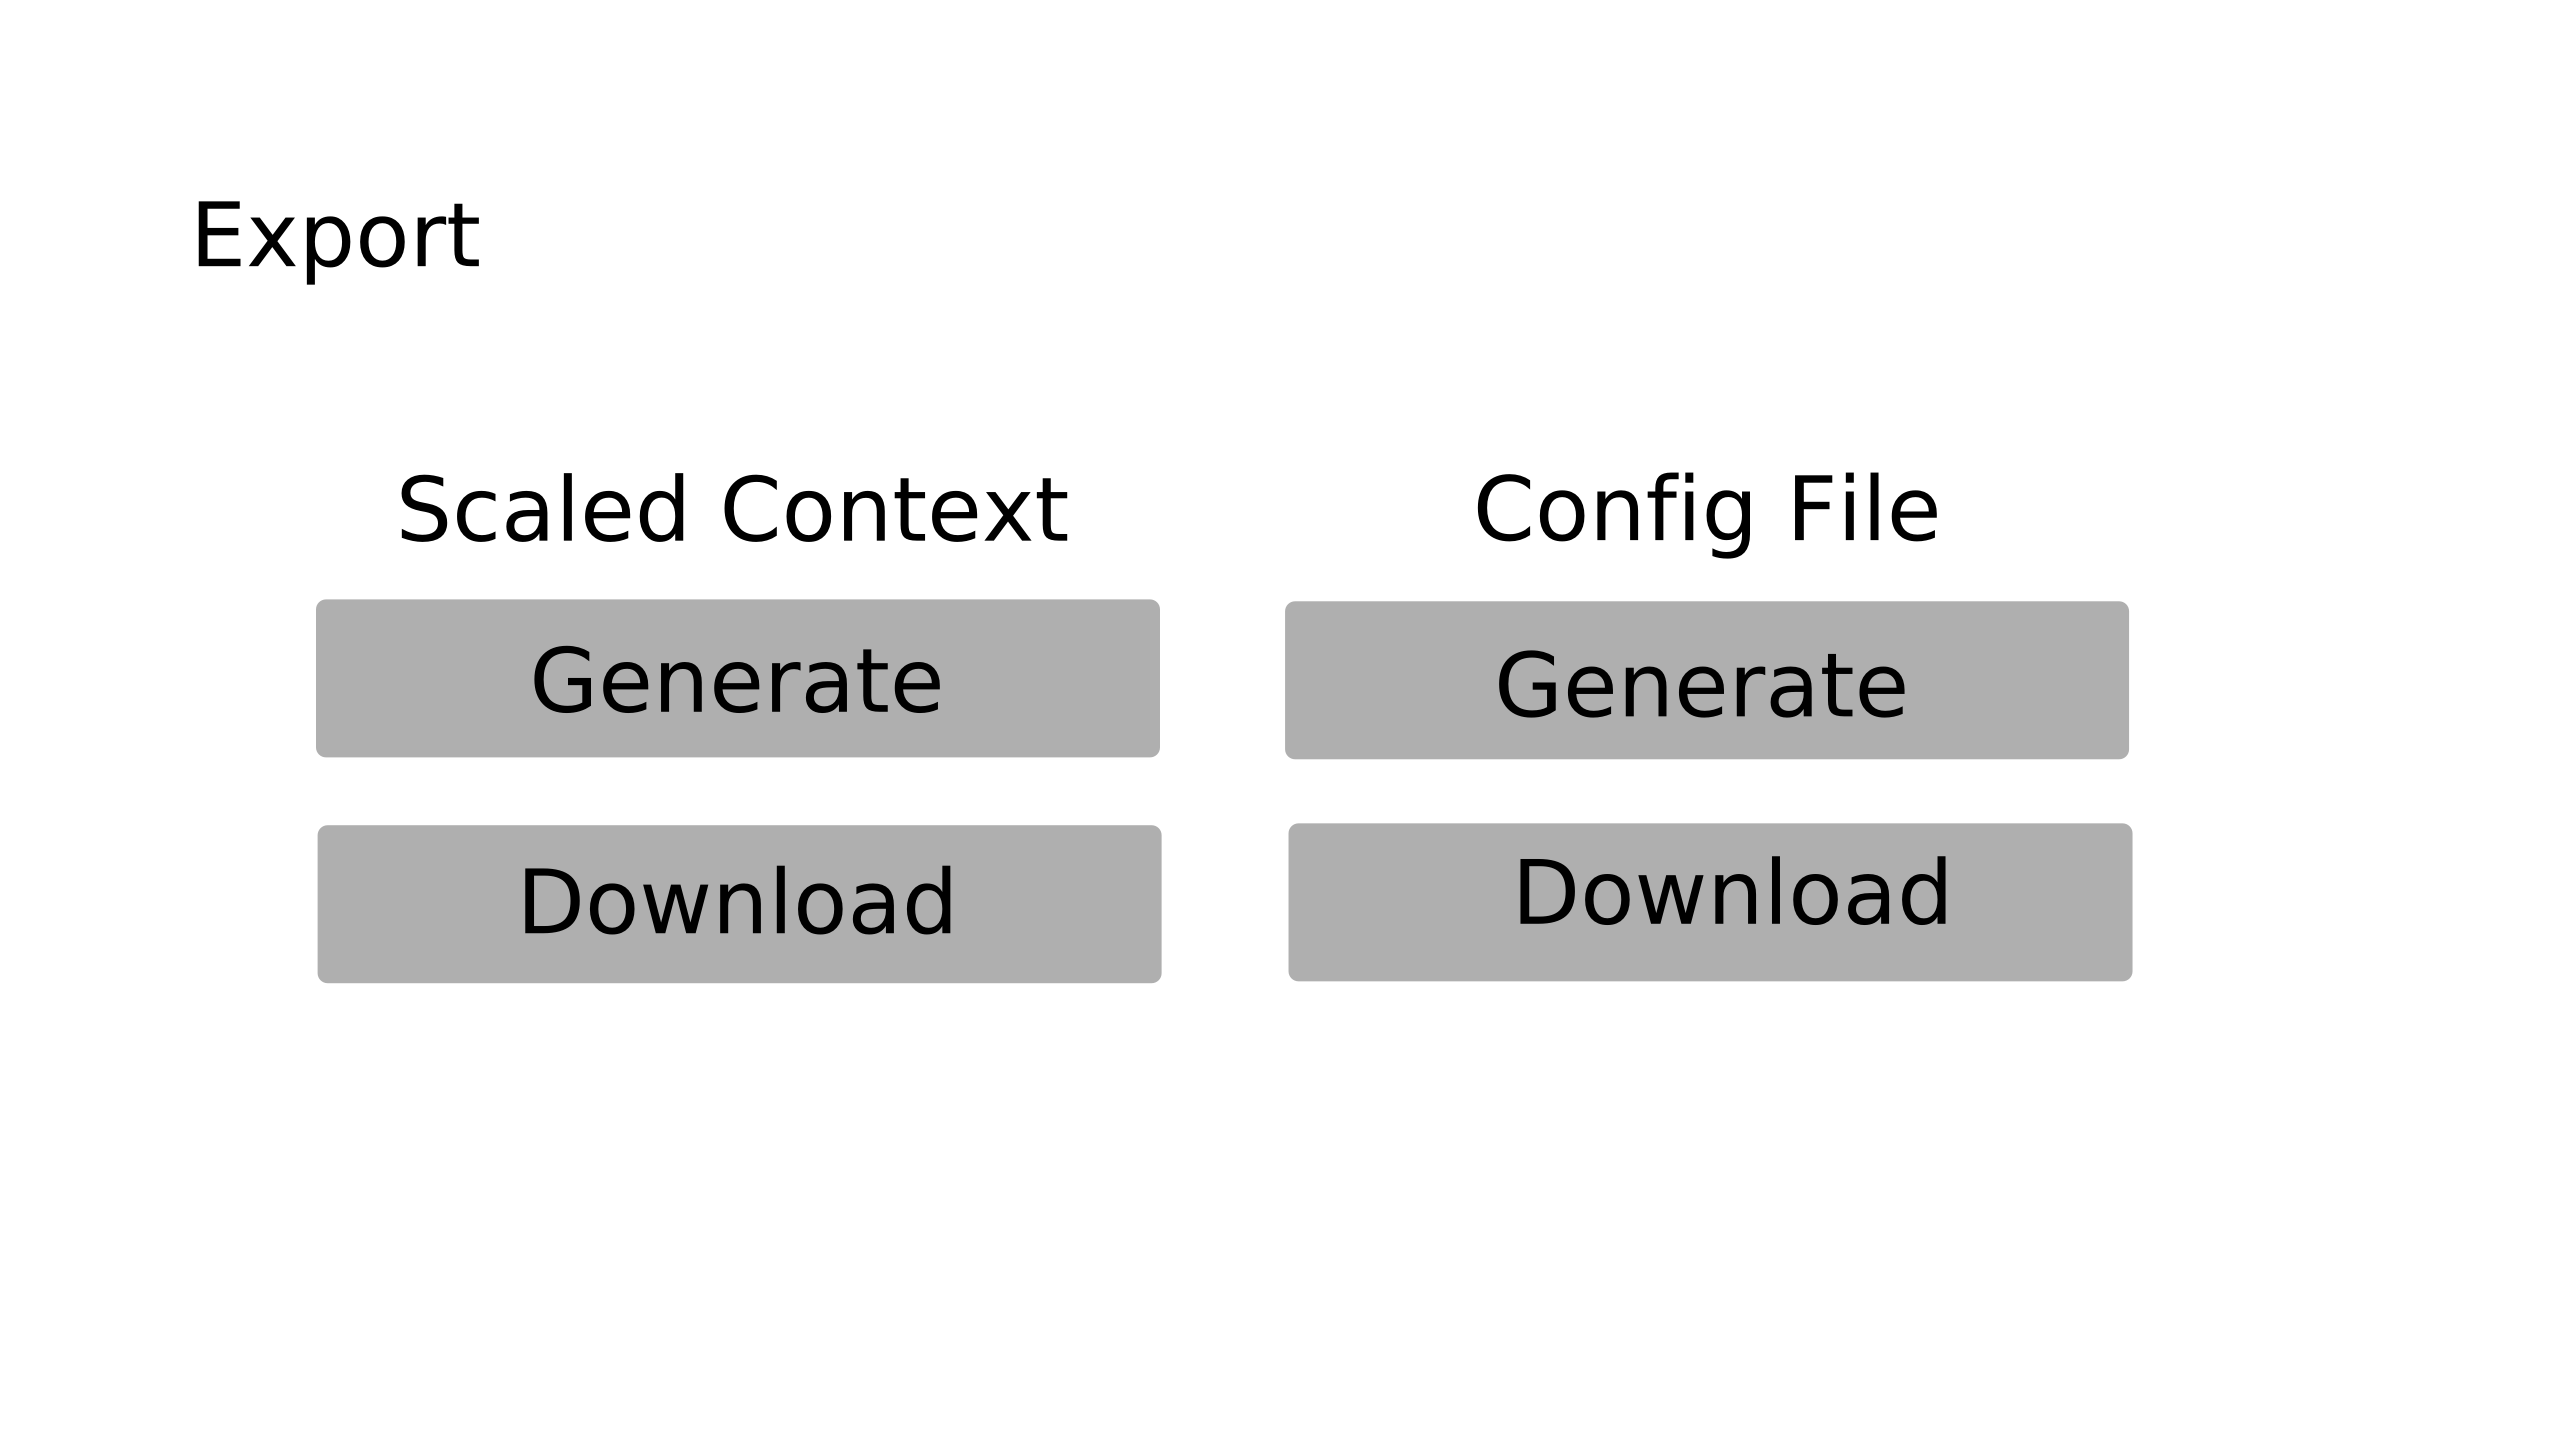
\includegraphics[width=\linewidth]{mock_up/export.png}
			\caption{Export panel}
			\label{fig:n1}
		\end{figure}
		\item Apply scales to mv-context and download it
		\item Context in Burmeister format
		\item Option to download .json config file to edit the scaling later
	\end{itemize}

\chapter{Implementation}
In very much the same order as before the now completed scaling tool is explained. The basic design remained the same but now there are much more details to cover. Each screen is presented with numerous markers and descriptions for everything clickable.

\section{Upload}
\begin{figure}[H]
	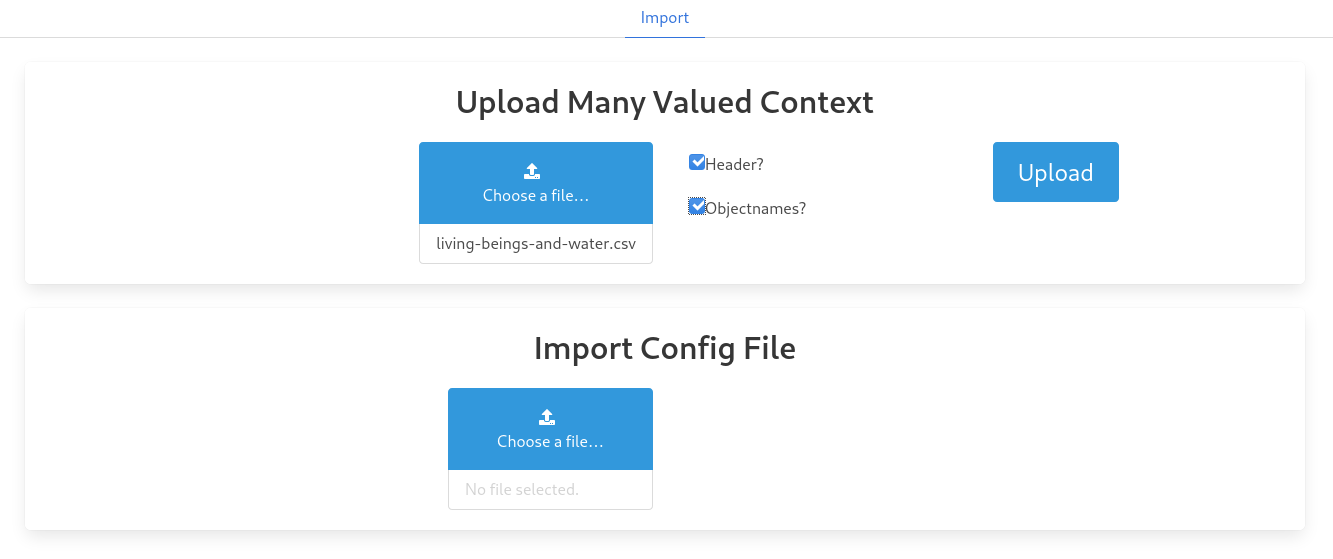
\includegraphics[width=\linewidth]{final_presentation/images/upload.png}
	\caption{The panel to select files}
	\label{fig:p1}
\end{figure}
\subsection{Features}
\begin{itemize}
    \item The topmost bar (Fig. ~\ref{fig:p1} A) allows for navigation and is updated with new panels whenever they get accessible.
	\item Select any local .csv file with a mv-context (Fig. ~\ref{fig:p1} B).
    \begin{itemize}
        \item There is the option to include a "header" (first line in file) with attribute names.
        \item "Objectnames" can be included in the first column of the file.
        \item To upload the file, click the "Upload"-button.
		\item Example .csv file with "header" and "objectnames"
		\begin{lstlisting}
				Age, Sex
PersonA, 30, m
PersonB, 25, d\end{lstlisting}
    \end{itemize}
    \item Additionally, you can edit already scaled contexts by importing config files (Fig. ~\ref{fig:p1} C) generated by the last panel in this document.
\end{itemize}

\section{Attribute-Selection}
\begin{figure}[H]
	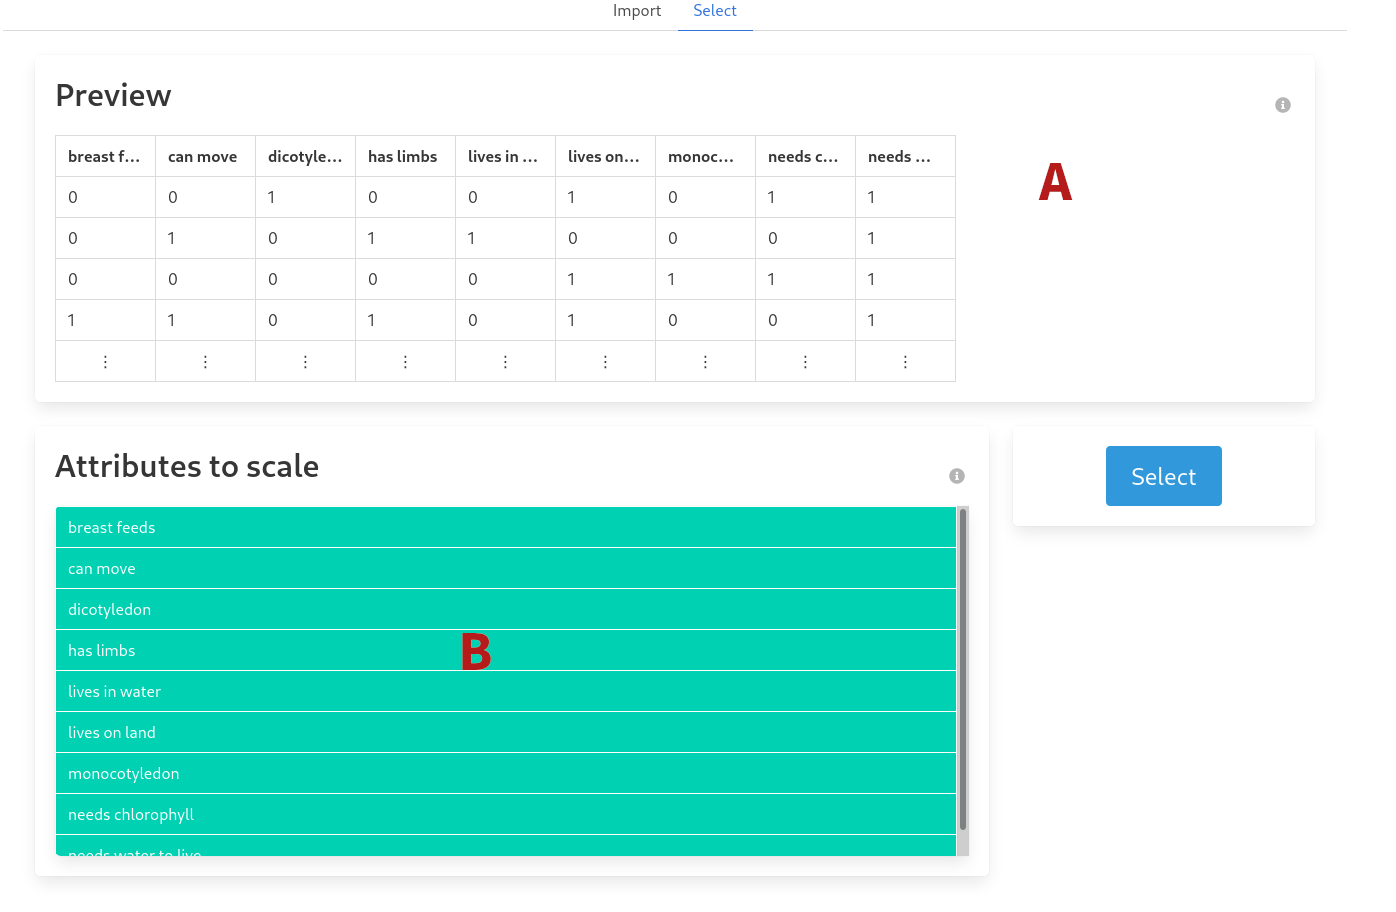
\includegraphics[width=\linewidth]{final_presentation/images/selection.png}
	\caption{The panel to select attributes}
	\label{fig:p2}
\end{figure}
\subsection{Features}
\begin{itemize}
    \item The top half (Fig. ~\ref{fig:p2} A) displays a preview of the uploaded data.
    \item The bottom half (Fig. ~\ref{fig:p2} B) allows for attributes to be selected for scaling. By default all attributes are selected (green) but can be unselected (white) with a click.
	\begin{itemize}
		\item By holding down the mouse button  multiple attributes can be de-/selected.
		\item Click "Select" to manually scale the chosen attributes.
	\end{itemize}
\end{itemize}

\section{Scaling}
\begin{figure}[H]
	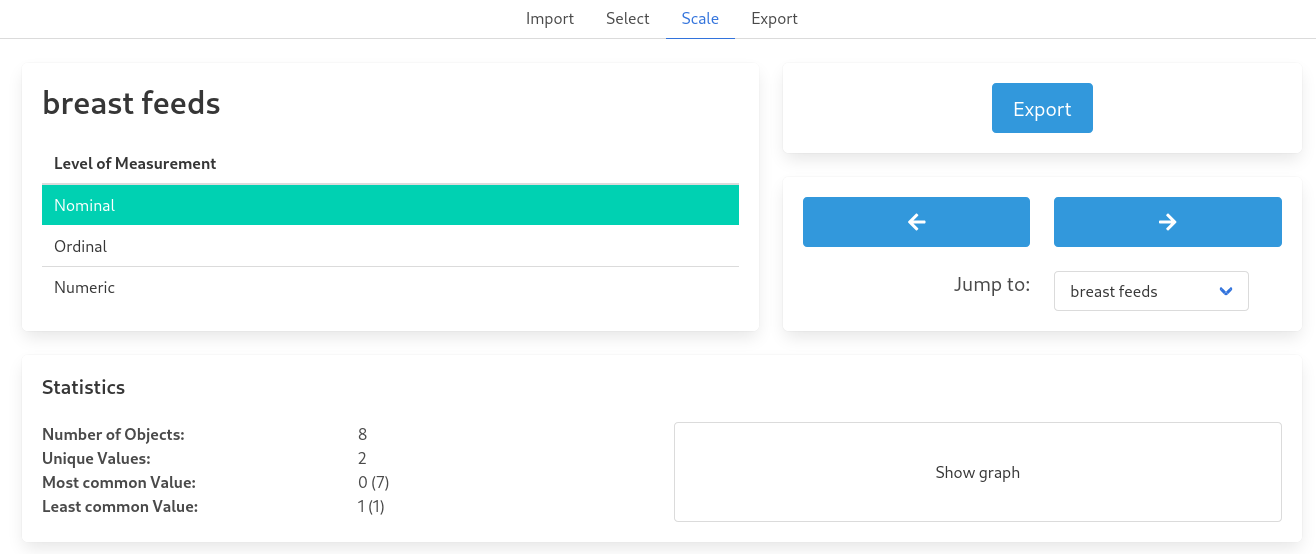
\includegraphics[width=\linewidth]{final_presentation/images/nominal.png}
	\caption{The panel to scale attributes}
	\label{fig:p3}
\end{figure}
\subsection{Features}
\begin{itemize}
    \item The top left half (Fig. ~\ref{fig:p3} A) allows for the selection of the scaling method for the current attribute (title). Based on the corresponding data some options may not be selectable.
    \begin{itemize}
        \item Subsequent sections will go into "Numeric" (Section 7) and "Ordinal" (Section 5-6) scaling, both of which will keep the header section as shown here. "Nominal" scaling is done automatically and therefore only consists of the header.
    \end{itemize}
    \item The top right half (Fig. ~\ref{fig:p3} B) allows for the "Export" of the scaled context. All unchanged attributes may be scaled nominally.
    \item Below the "Export" (Fig. ~\ref{fig:p3} C) one can change the current attribute.
    \item Each scaling method shows "Statistics" (Fig. ~\ref{fig:p3} D) relevant for the scaling and the option for a graph.
\end{itemize}

\section{Scaling Graph}
\begin{figure}[H]
	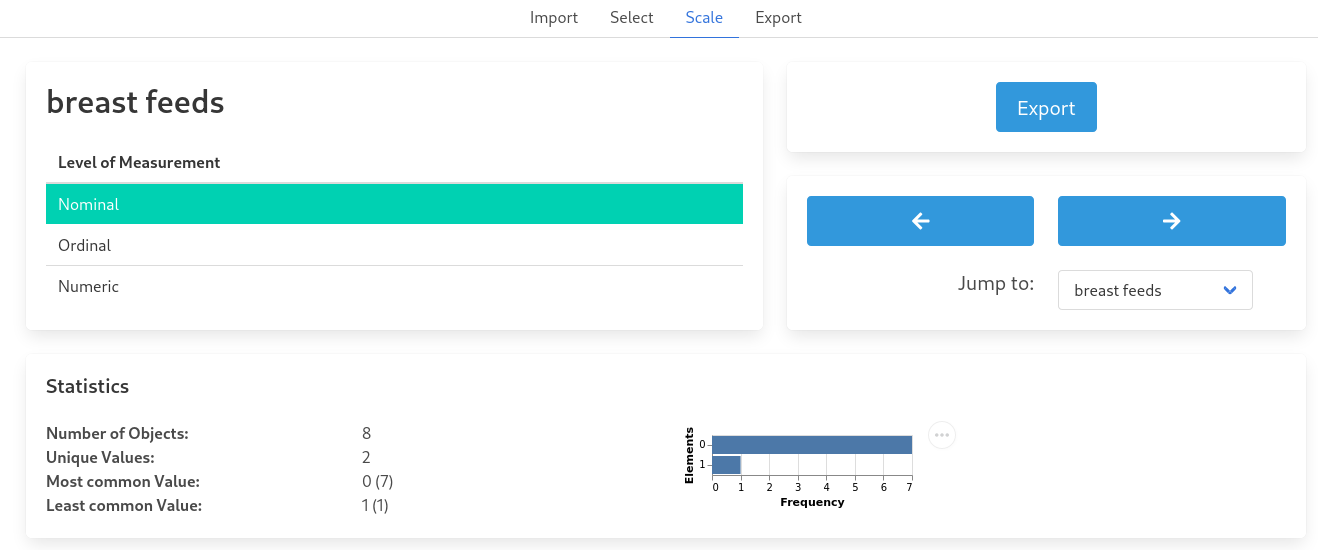
\includegraphics[width=\linewidth]{final_presentation/images/nominal_graph.png}
	\caption{The panel to select attributes}
	\label{fig:p4}
\end{figure}
\subsection{Features}
\begin{itemize}
    \item By clicking the button (shown in Fig. ~\ref{fig:p3} D)  a temporary graph is generated (Fig. ~\ref{fig:p4} A). The graph will disappear upon changing the scaling method or upon changing the current attribute and has to be generated again.
\end{itemize}

\newpage
\section{Ordinal Scaling}
\begin{figure}[H]
	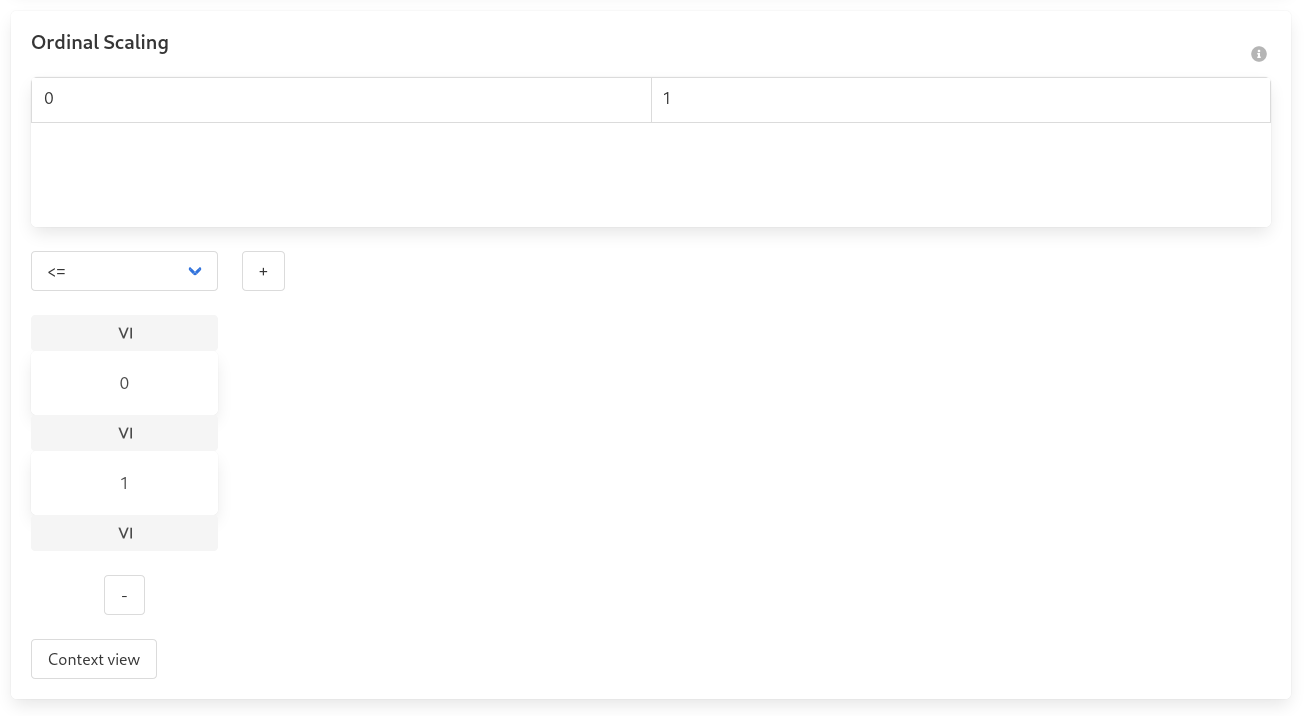
\includegraphics[width=\linewidth]{final_presentation/images/ordinal.png}
	\caption{The panel to scale ordinal attributes}
	\label{fig:p5}
\end{figure}
\subsection{Features}
\begin{itemize}
    \item The default option to perform ordinal scaling is to build orders from the possible values.
    \item The box on top of the panel (Fig. ~\ref{fig:p5} A) contains each different value the attribute has.
    \item Below a new order can be created either by clicking the "+" (Fig. ~\ref{fig:p5} B) or by dragging values from the box above on the "+"-button.
    \begin{itemize}
        \item Each order (Fig. ~\ref{fig:p5} C) has a drop-down menu were an order relation can be selected.
        \item By dragging values onto the grey areas the value is inserted into the order.
        \item Values can also be dragged out of the order or into different positions by dragging the white box of the corresponding value.
    \end{itemize}
    \item The "Context view"-button transforms the current orders into a context and changes the panel.
\end{itemize}

\section{Ordinal Context Scaling}
\begin{figure}[H]
	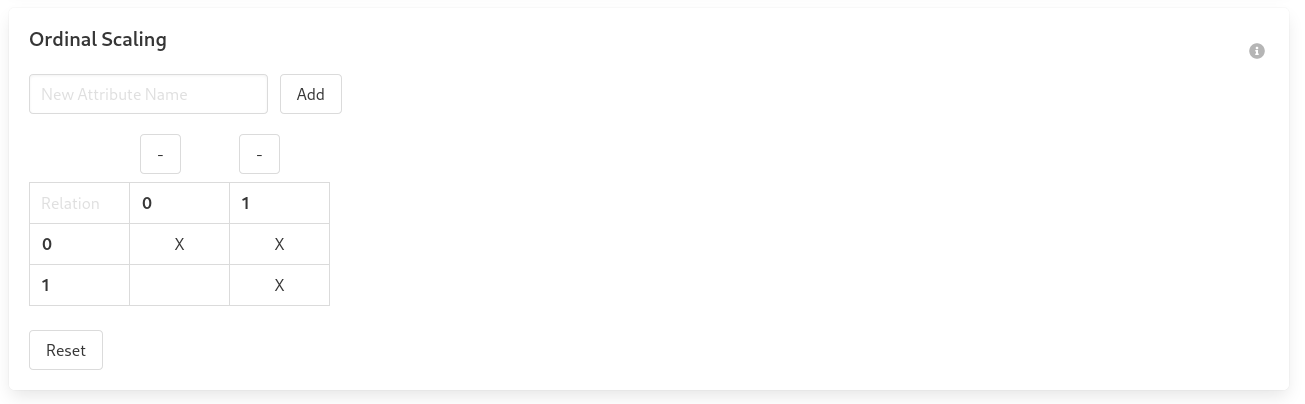
\includegraphics[width=\linewidth]{final_presentation/images/ordinal_ctx.png}
	\caption{The second panel to scale ordinal attribute}
	\label{fig:p6}
\end{figure}
\subsection{Features}
\begin{itemize}
    \item Per default the generated context is quadratic (Fig. ~\ref{fig:p6} B) and contains all orders previously built.
    \item New attributes can be generated by writing their name in the topmost input field and clicking "Add" (Fig. ~\ref{fig:p6} B). Clicking the "-" removes the attribute below it.
    \item Attributes and objects can be sorted with drag and drop.
    \item The top left corner allows to name the relation used which is purely cosmetic.
    \item To swap a relation between " " and "x" click the corresponding field.
    \item "Reset" discards all changes done to the context and return to the previous panel with all orders built before.
\end{itemize}

\section{Numeric Scaling}
\begin{figure}[H]
	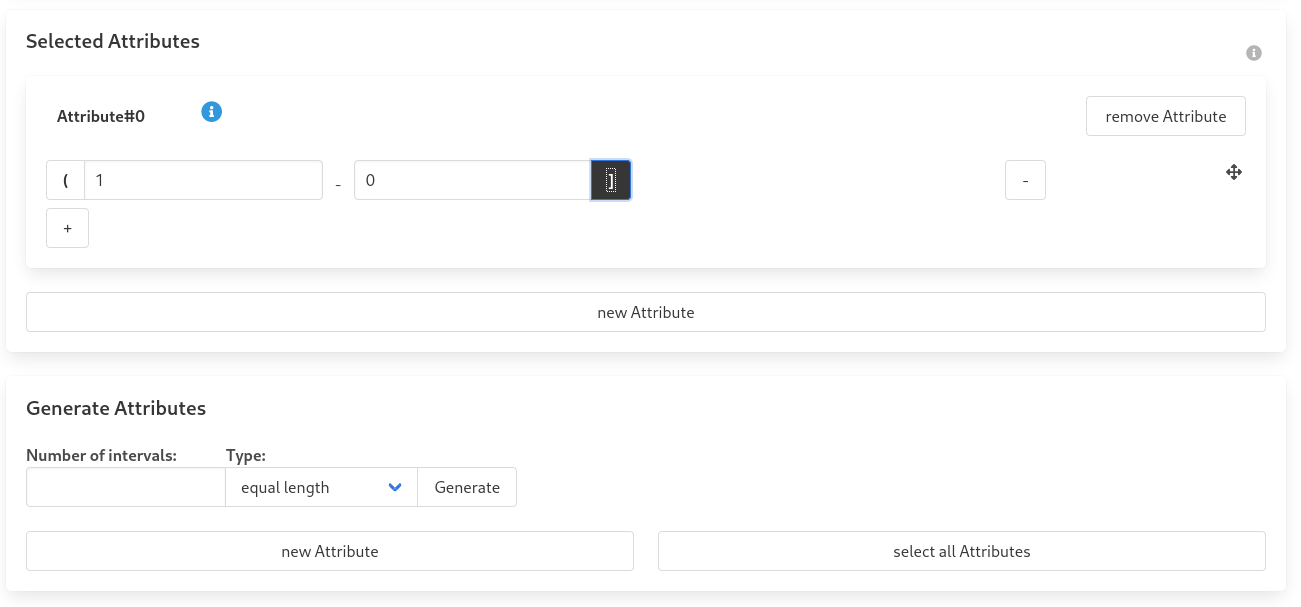
\includegraphics[width=\linewidth]{final_presentation/images/numeric.png}
	\caption{The panel to scale numeric attributes.}
	\label{fig:p7}
\end{figure}
\subsection{Features}
\begin{itemize}
    \item The upper panel (Fig. ~\ref{fig:p7} A) contains all selected attributes.
    \begin{itemize}
        \item "new Attribute" and "remove Attribute" add/delete attributes. 
        \item The attribute name can be clicked and written in to change it.
        \item "+" and "-" add/delete intervals (Fig. ~\ref{fig:p7} C) from an attribute.
        \item A value is added to an attribute if it is contained in one of its intervals. The interval can be toggled to be open ("(") and closed ("]") by clicking the brackets.
        \item Intervals can moved to other attributes by drag and drop.
    \end{itemize}
    \item The lower panel (Fig. ~\ref{fig:p7} B) generates attributes.
    \begin{itemize}
        \item By clicking "Generate" the written number of intervals is generated by the selected method from the drop-down menu.
        \item Those attributes must be selected to be used by clicking "Select" or "Select all". Selected Attributes are moved to the upper half.
    \end{itemize}
\end{itemize}

\section{Export panel}
\begin{figure}[H]
	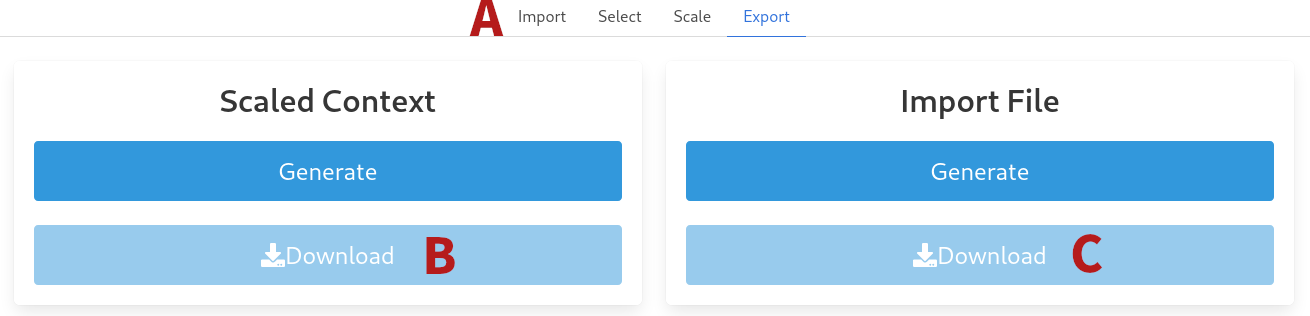
\includegraphics[width=\linewidth]{final_presentation/images/export.png}
	\caption{The panel to export the scaled context}
	\label{fig:p8}
\end{figure}
\subsection{Features}
\begin{itemize}
	\item On top is the navigation bar with all possible entries (Fig. ~\ref{fig:p8} A). 
    \item By clicking the corresponding button an import file and a scaled context can be "generated".
    \item The scaled context applies all chosen scales to the selected attributes and outputs the context in "Burmeister"-format (Fig. ~\ref{fig:p8} B) .
    \item The import file (Fig. ~\ref{fig:p8} C) consists of a .json file with the current state of the application. This file can later be used to change the different scaling methods applied to the attributes or to change the selected attributes.
\end{itemize}

\chapter{Conclusion}
The resulting tool both followed the initial timetable and the mock-up almost perfectly. Each of the different scaling methods received a matching user interface with rather simple instructions provided for each. While nominal scaling is done completely automatic, all other cases of ordinal scaling are implemented by building different orders of elements. This follows the rule that all concept lattices can be disjoint into linear orders. Additionally the resulting context can be edited directly. Numeric scaling is based on building new attributes from multiple assigned intervals, both inclusive and exclusive. While all of these options provide are more easy to use user interface than available before, the usability is also the most important goal to iterate upon in the future. Currently the tool still misses some options to simplify the scaling of larger contexts. Nominal scaling works automatic regardless of the initial size and numeric scaling features the automatic generation of intervals, but ordinal scaling lacks such a feature. Both the simple interface and the direct editing of the context would greatly benefit from a multi-select option or initial orders.

\end{document}
